\documentclass{article}

% Language setting
% Replace `english' with e.g. `spanish' to change the document language
\usepackage[english]{babel}

% Set page size and margins
% Replace `letterpaper' with `a4paper' for UK/EU standard size
\usepackage[letterpaper,top=2cm,bottom=2cm,left=3cm,right=3cm,marginparwidth=1.75cm]{geometry}

% Useful packages

\usepackage{comment}
\usepackage{amsmath}
\usepackage{graphicx}
\usepackage{algorithm}
\usepackage{algpseudocode}
\usepackage{booktabs}
\usepackage{pdflscape} % Add this package for landscape pages
\usepackage{caption,subcaption}
\usepackage[colorlinks=true, allcolors=blue]{hyperref}
% \setcounter{section}{4}
\setcounter{subsection}{4}
\title{Assignment 5}
\author{Megan Mirnalini SundaramR, Sherry Usman}

\begin{document}
\maketitle


\section*{Part 5.1}
\subsection*{Segmentation of the Embryos}
\textbf{Note:} Some of the images (e.g. images 21, 24, 26) have been combined to produce a better image. \newline This has been discussed in \ref{Appendix A}.
To use the images for segmentation of embryos, they first need to be pre-processed to enhance their quality. The algorithm for pre-processing is listed as Algorithm 1.
\begin{algorithm}[h!]
\caption{Pre-processing Images}\label{algo:pre-processing-images}
\begin{algorithmic}[1]
\Procedure{ImageProcessing}{$\text{images}$}
    \For{$\text{image}$ \textbf{in} $\text{images}$}
        \State $gray\_image \gets \text{Grayscale}(image)$
        \State $image\_contrasted \gets \text{ContrastStretch}(image)$
        \State $image\_thresholded \gets \text{RangeThreshold}(image\_contrasted)$
        \State $image\_eroded \gets \text{Eroded}(image\_thresholded)$
        \State $image\_dilated \gets \text{Eroded}(image\_eroded)$
        \State $image\_inverted \gets \text{Inverted}(image\_dilated)$
        \State $image\_opened \gets \text{Opening}(image\_inverted)$
        \State $image\_eroded \gets \text{Eroded}(image\_opening)$
        \State $gray\_image \gets \text{Grayscale}(image\_eroded)$
    \EndFor
    \State \textbf{return} Gray Image
\EndProcedure
\end{algorithmic}
\end{algorithm}

As seen in algorithm \ref{algo:pre-processing-images}, the image is first converted to a gray-scale image, so that it can be processed further. This image is then contrast-stretched with a lower-bound of 70 and an upper-bound of 100, so as to correct image exposure. The contrast-stretched image is then dilated by 5.75, so as to remove the breaks and intrusions in the image. This dilated image is then inverted and opened by a structuring element of size 10. This is done to smooth the boundaries of the image and help to reverse some of the effects of the previous erosion. 

\subsection*{Panel of the Original Images}
In order to prepare a panel of the original and binary images, the images had to be resized and cropped to remove the spaces in the image, and highlight the embryo. The technique is highlighted in Algorithm \ref{algo:bounding-box}.  
\begin{algorithm}[h!]
\caption{Get the Bounding Box For The Embryos Images}\label{algo:bounding-box}
\begin{algorithmic}[1]
\Procedure{BoundingBoxForEmbryos}{$\text{processed\_images}$}
    \For{$\text{image}$ \textbf{in} $\text{processed\_images}$}
        \State $CannyProcessedImage \gets \text{CannyEdgeDetection}(\text{image})$
        \State $edge\_points \gets \text{NonZeroPoints}(CannyProcessedImage)$
        \State $z\_score \gets \text{computeZscore}(edge\_points)$
        \State $filtered\_points \gets \text{RemoveOutliers}(edge\_points)$
        \State $(\text{minimum\_x}, \text{minimum\_y}) \gets \text{Minimum}(filtered\_points)$
        \State $(\text{maximum\_x}, \text{maximum\_y}) \gets \text{Maximum}(filtered\_points)$
    \EndFor
    \State $\text{width} \gets \text{maximum\_x} - \text{minimum\_x}$
    \State $\text{height} \gets \text{maximum\_y} - \text{minimum\_y}$
    \State \textbf{return} $\text{minimum\_x}$, $\text{minimum\_y}$, $\text{width}$, $\text{height}$ 
\EndProcedure
\end{algorithmic}
\end{algorithm}

The above algorithm used Canny Edge Detection technique to detect the edges (sharp changes of intensity going from foreground to background) of the embryos. The Z score of edge points is then computed to find potential outliers or anomalies in edge points. The outliers are then removed in RemoveOutliers function and then from the remaining points  we can calculate the maximum x and y values and the minimum x and y values to create an approximate bounding box that encompasses the whole object. \\The dimensions are then, used to crop the image. The cropped images are then, displayed in a 4*15 grid (shown in figure \ref{fig:panel-original}). 

\subsection*{Panel of the Binary Images}
Similarly, the output of Algorithm \ref{algo:pre-processing-images} is displayed in a 4*15 grid (shown in figure \ref{fig:panel-binary}). 
\begin{landscape}
    \begin{figure}
    \centering
    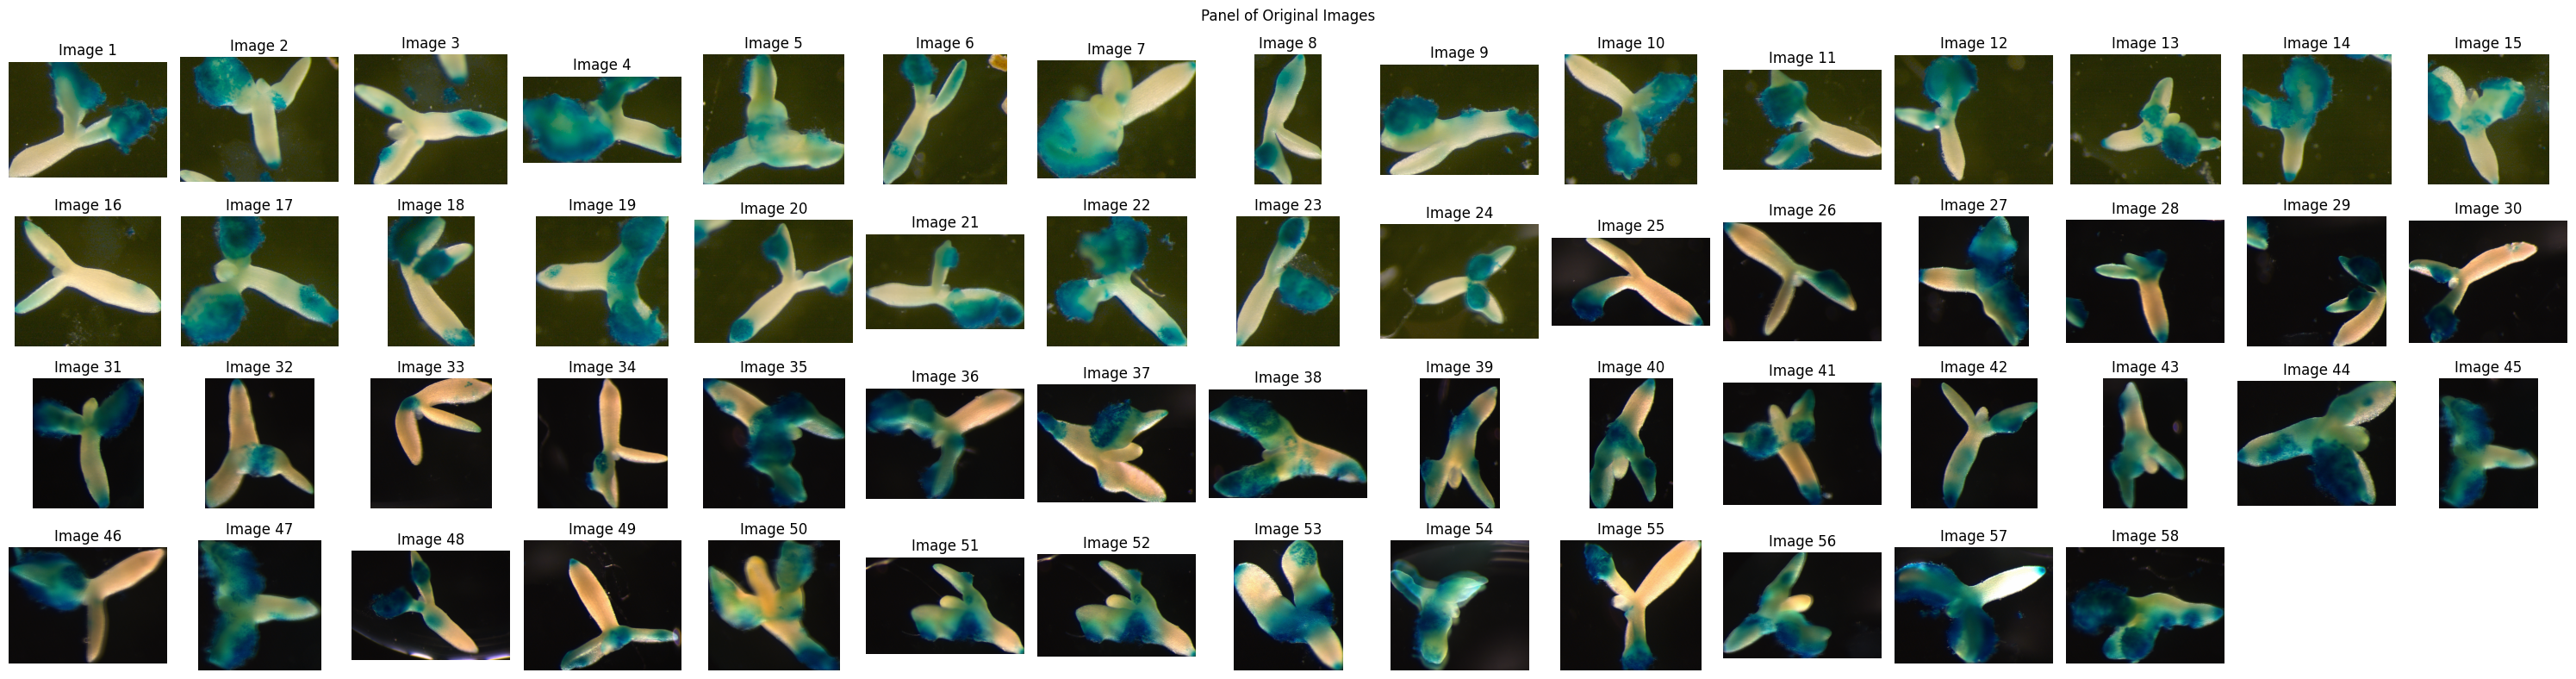
\includegraphics[width=1\linewidth, keepaspectratio]{Report/Images/Panel_of_Original_Images.png}
    \caption{A panel of 4*15 containing the cropped original images}
    \label{fig:panel-original}
\end{figure}
\end{landscape}
\clearpage
\begin{landscape}
    \begin{figure}
    \centering
    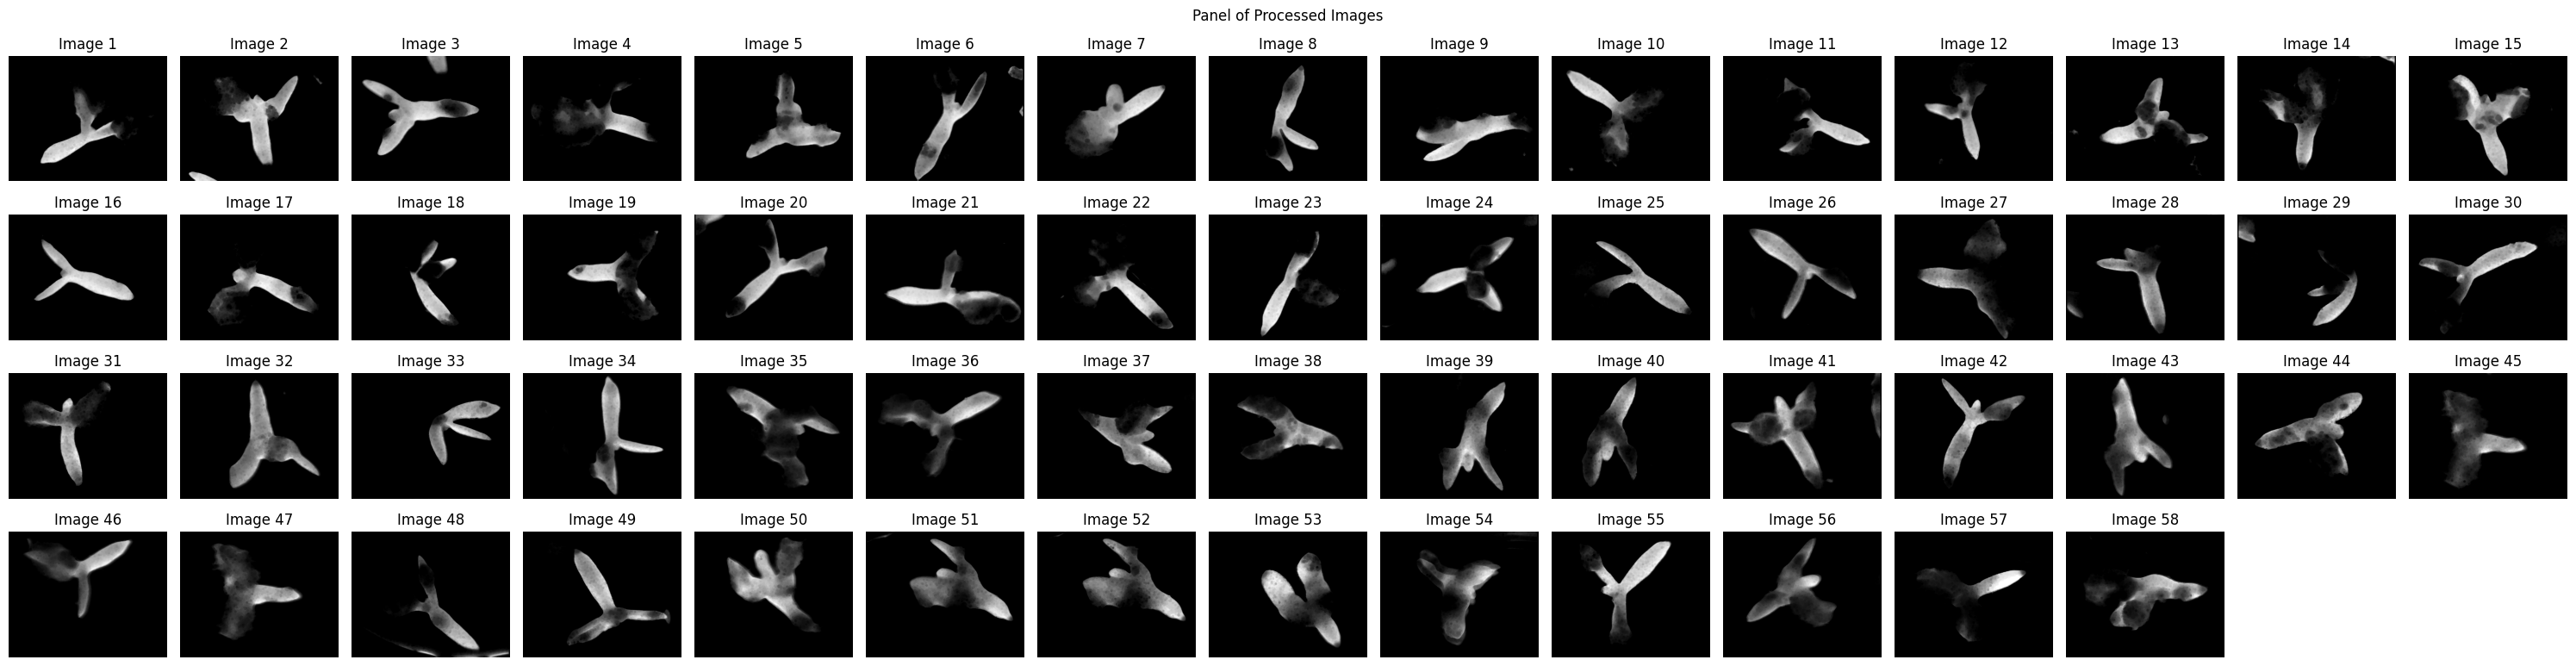
\includegraphics[width=1\linewidth, keepaspectratio]{Report/Images/Panel_of_Processed_Images.png}
    \caption{A panel of 4*15 containing the processed gray-scale images}
    \label{fig:panel-binary}
\end{figure}
\end{landscape}
\clearpage
\section*{Part 5.2}
\subsection*{Size and Shape of the Embryos}
In order to compute the amount of gene-expression in the embryo, it is essential to segment the embryos shown in the images into two parts - one containing the blue portion (which indicates the gene expression) and the other containing the rest of the embryo. Then the area of the blue part can be subtracted from the area of the whole object/embryo to find the area of non-blue/yellow part. This is done to accurately estimate the level of gene-expression and to determine features such as size, shape etc. 

Firstly, the images are taken and processed based on the color range. 
\begin{algorithm}[h!]
\caption{Processing Colors in the Embryos}\label{algo:processing_colors}
\begin{algorithmic}[1]
\Procedure{ImageProcessing}{$\text{images}$}
    \State $\text{closest\_row[figure]} \gets \text{empty list}$
    \For{$\text{image}$ \textbf{in} $\text{images}$}
        \State $gray\_image \gets \text{Grayscale}(\text{image})$
        \State $image\_contrasted \gets \text{ContrastStretch}(gray\_image)$
        \State $yellow\_part \gets \text{YellowRangeThreshold}(image\_contrasted)$
        \State $cleaned\_yellow\_part \gets \text{MedianFilter}(image\_contrasted)$
        \State $eroded\_image \gets \text{Erosion}(image\_contrasted)$
        \State $whole\_image \gets \text{RangeThreshold}(eroded\_image)$
        \State $cleaned\_whole\_image \gets \text{MedianFilter}(whole\_image)$
        \State $blue\_part \gets \text{(difference)}((whole\_image),(yellow\_image))$
        \State $cleaned\_blue\_part \gets \text{MedianFilter}(blue\_part)$
    \EndFor
    \State \textbf{return} GrayImage, YellowPart, BluePart
\EndProcedure
\end{algorithmic}
\end{algorithm}

The image is first converted to a grayscale image. From this, the image is contrast stretched to a lower-bound value of 50 and an upper-bound value of 100. \\Firstly, the yellow part i.e., the remaining part of the embryo is computed. This is done by range-thresholding the image from 50 to 250, to extract the yellow part of the image. A median filter is applied to this, to remove the noise and clean the image. This constitutes the yellow part of the image. 
\par Similarly, the contrast-stretched image is eroded by a factor of 5, to remove the extrusions. The eroded image, is then range-thresholded from a range of 5 to 255 (to remove glare, and retain other parts of the image). This constitutes the whole image. 
\par Finally, the blue part of the image, i.e., the gene-expression is obtained by the difference of the entire image, and the yellow part of the image. This is then subjected to a median fiter, to clean the image. This constitutes the blue part of the image. \\The output of this algorithm is shown in figures \ref{fig:segment1-4},\ref{fig:segment5-8},\ref{fig:segment9-12}, \ref{fig:segment13-16}, \ref{fig:segment17-20}, \ref{fig:segment21-24}, \ref{fig:segment25-28}, \ref{fig:segment29-32}, \ref{fig:segment33-36}, \ref{fig:segment37-40}, \ref{fig:segment41-44}, \ref{fig:segment45-48}, \ref{fig:segment49-52}, \ref{fig:segment53-56} and \ref{fig:segment57-58}.

The size and shape of the embryo is then, calculated with the help of the blue part of the segmented image. The results are tabulated below in tables \ref{tab:size_shape_embryo_pt1} and \ref{tab:size_shape_embryo_pt2}.
\begin{table}[h!]
    \centering
    \begin{tabular}{|c|c|c|c|}
    \hline
    Image & Size of the Embryo & Size of the Gene Expression & Relative Proportion \\  \hline
    1 & 200640 & 64650 & 0.322 \\     \hline
    2 & 267696 & 44085 & 0.165 \\    \hline
    3 & 236810 & 7230 & 0.031 \\    \hline
    4 & 307462 & 147813 & 0.481 \\    \hline
    5 & 215819 & 15594 & 0.072 \\    \hline
    6 & 220675 & 41845 & 0.19  \\    \hline
    7 & 256440 & 22588 & 0.088  \\    \hline
    8 & 160677 & 17912 & 0.111  \\    \hline
    9 & 228927 & 48672 & 0.213  \\    \hline
    10 & 247231 & 72798 & 0.294  \\    \hline
    11 & 178070 & 47816 & 0.269  \\    \hline
    12 & 168141 & 53765 & 0.32  \\    \hline
    13 & 218581 & 48398 & 0.221  \\ \hline
    14 & 260238 & 101286 & 0.389 \\    \hline
    15 & 288132 & 43375 & 0.151 \\    \hline
    16 & 148619 & 193 & 0.001 \\    \hline
    17 & 237325 & 81726 & 0.344 \\    \hline
    18 & 121812 & 18307 & 0.15 \\    \hline
    19 & 223586 & 100185 & 0.448 \\    \hline
    20 & 215391 & 34001 & 0.158 \\    \hline
    21 & 254119 & 67299 & 0.265 \\    \hline
    22 & 287164 & 119959 & 0.418 \\\hline
    23 & 196536 & 70916 & 0.361 \\    \hline
    24 & 241160 & 70267 & 0.291 \\    \hline
    25 & 237813 & 92183 & 0.388 \\    \hline
    26  & 192618 & 31906 & 0.166 \\    \hline
    27 & 308532 & 130611 & 0.423  \\    \hline
    28 & 189985 & 42675 & 0.225  \\    \hline
    29 & 142909 & 40508 & 0.283  \\    \hline
    30 & 226351 & 76089 & 0.336  \\    \hline
    31 & 220285 & 116666 & 0.53 \\  \hline
    32 & 226098 & 5667 & 0.025 \\ \hline
    33 & 142437 & 6474 & 0.045 \\ \hline
    34 & 185253 & 18968 & 0.102 \\ \hline
    35 & 298102 & 161233 & 0.541 \\ \hline
    36 & 271587 & 110394 & 0.406 \\ \hline
    37 & 235880 & 55366 & 0.235 \\ \hline
    38 & 220593 & 76127 & 0.345 \\ \hline
    39 & 221785 & 29674 & 0.134 \\ \hline
    40 & 212481 & 73694 & 0.347 \\ \hline
    \end{tabular}
    \caption{Size and Shape of Gene Expression for the first 40 images}
    \label{tab:size_shape_embryo_pt1}
\end{table}

\begin{table}[h!]
    \centering
    \begin{tabular}{|c|c|c|c|}
    \hline
    Image & Size of the Embryo & Size of the Gene Expression & Relative Proportion \\  \hline
    41 & 333242 & 94048 & 0.282 \\ \hline
    42 & 180554 & 25225 & 0.14 \\ \hline
    43 & 230685 & 52560 & 0.228 \\ \hline
    44 & 252624 & 64132 & 0.254 \\ \hline
    45 & 287818 & 147962 & 0.514 \\ \hline
    46 & 223816 & 77331 & 0.346 \\ \hline
    47 & 280804 & 127458 & 0.454 \\ \hline
    48 & 226735 & 89915 & 0.397 \\ \hline
    49 & 229402 & 36738 & 0.16 \\ \hline
    50 & 284019 & 45775 & 0.161 \\ \hline
    51 & 260636 & 40011 & 0.154 \\ \hline
    52 & 258195 & 38355 & 0.149 \\ \hline
    53 & 260940 & 30439 & 0.117 \\ \hline
    54 & 390661 & 190844 & 0.489 \\ \hline
    55 & 211979 & 43190 & 0.204 \\ \hline
    56 & 240496 & 52318 & 0.218 \\ \hline
    57 & 266155 & 152484 & 0.573 \\ \hline
    58 & 282389 & 141063 & 0.5 \\ \hline
    \end{tabular}
    \caption{Size and Shape of Gene Expression for the last 18 images}
    \label{tab:size_shape_embryo_pt2}
\end{table}

In addition to this, the texture i.e., uniformity and standard deviation of the embryo was also computed. 
\begin{figure}[h!]
    \centering
    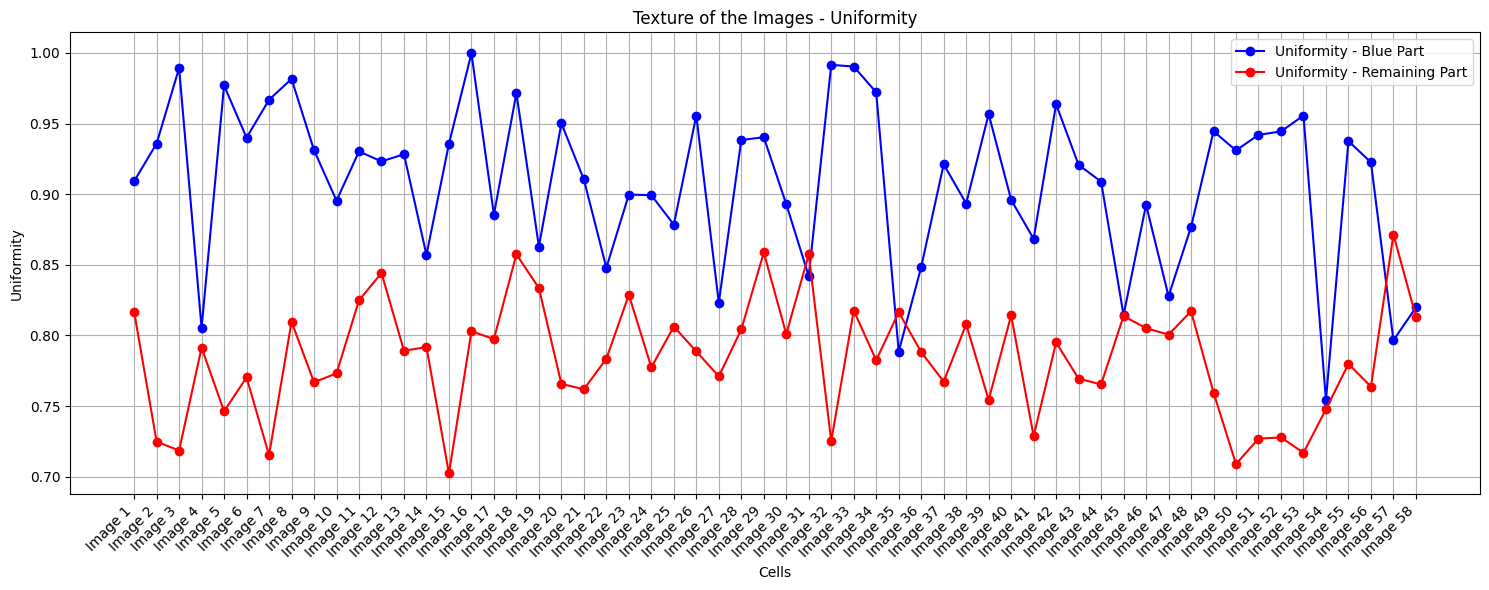
\includegraphics[width=1\linewidth]{Report/Images/Texture_Segments_Uniformity.png}
    \caption{Uniformity of the Embryos}
    \label{fig:embryo_uniformity}
\end{figure}
\begin{figure}[h!]
    \centering
    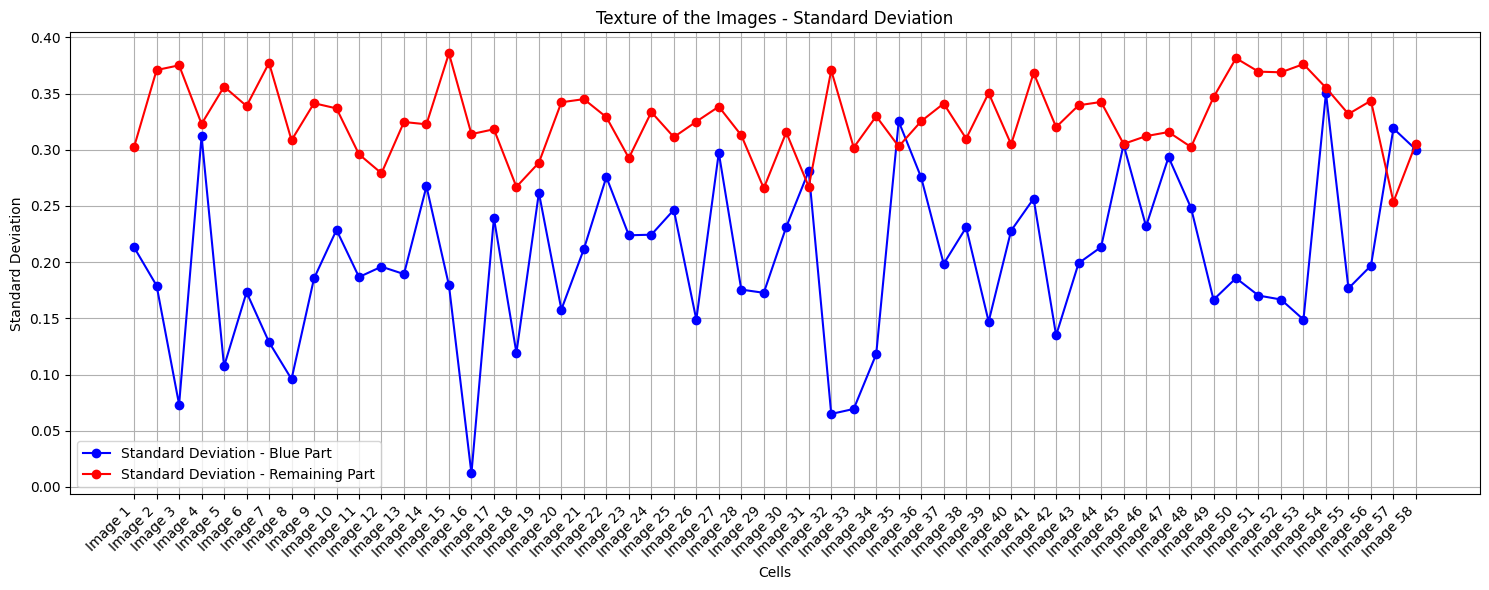
\includegraphics[width=1\linewidth]{Report/Images/Texture_Segments_StandardDeviation.png}
    \caption{Uniformity of the Embryos}
    \label{fig:embryo_uniformity}
\end{figure}
The size and shape of the embryos was measured using the in-built functions and are tabulated in \ref{tab:size_shape_embryo_pt1} and \ref{tab:size_shape_embryo_pt2} .
\begin{table}[h!]
    \centering
    \begin{tabular}{|c|c|c|c|c|c|}
    \hline
        Image  &  Object Count  &  Size  &  Perimeter  &  Solidity  &  Convexity \\ \hline
        1  &  35  &  990.914  &  117.064  &  0.722  &  0.966  \\ \hline
        2  &  37  &  1261.865  &  183.545  &  0.801  &  0.958 \\ \hline
        3  &  33  &  941.667  &  216.071  &  0.72  &  0.932 \\ \hline
        4  &  41  &  637.927  &  66.895  &  0.897  &  0.971 \\ \hline
        5  &  10  &  9059.5  &  637.97  &  0.719  &  0.918 \\ \hline
        6  &  14  &  4793.429  &  436.73  &  0.776  &  0.901 \\ \hline
        7  &  5  &  12031.6  &  547.944  &  0.73  &  0.937 \\ \hline
        8  &  32  &  1233.594  &  156.68  &  0.802  &  0.934 \\ \hline
        9  &  45  &  767.622  &  105.64  &  0.744  &  0.971 \\ \hline
        10  &  5  &  8832  &  758.33  &  0.698  &  0.825 \\ \hline
        11  &  34  &  605.353  &  113.772  &  0.811  &  0.952 \\ \hline
        12  &  12  &  2226.917  &  242.351  &  0.667  &  0.913 \\ \hline
        13  &  17  &  2920.647  &  260.641  &  0.783  &  0.947 \\ \hline
        14  &  12  &  3989.333  &  266.032  &  0.749  &  0.898 \\ \hline
        15  &  8  &  9948  &  536.231  &  0.668  &  0.923 \\ \hline
        16  &  134  &  55.418  &  33.793  &  0.854  &  0.984 \\ \hline
        17  &  33  &  735.424  &  118.219  &  0.813  &  0.952 \\ \hline
        18  &  26  &  654.385  &  140.229  &  0.699  &  0.948 \\ \hline
        19  &  4  &  4736.75  &  494.872  &  0.551  &  0.947 \\ \hline
        20  &  9  &  5168.222  &  647.139  &  0.724  &  0.928 \\ \hline
        21  &  13  &  2751.385  &  389.688  &  0.853  &  0.928 \\ \hline
        22  &  9  &  3706.333  &  408.243  &  0.64  &  0.92 \\ \hline
        23  &  15  &  1425.4  &  230.114  &  0.604  &  0.946 \\ \hline
        24  &  7  &  4379.429  &  608.36  &  0.559  &  0.874 \\ \hline
        25  &  78  &  417.103  &  72.526  &  0.808  &  0.967 \\ \hline
        26  &  4  &  14467.5  &  829.635  &  0.745  &  0.921 \\ \hline
        27  &  14  &  3410.714  &  313.918  &  0.791  &  0.913 \\ \hline
        28  &  14  &  5666.643  &  271.421  &  0.848  &  0.952 \\ \hline
        29  &  28  &  1255.25  &  149.904  &  0.845  &  0.936 \\ \hline
        30  &  52  &  574.615  &  89.039  &  0.776  &  0.978 \\ \hline
        31  &  11  &  5162  &  219.242  &  0.829  &  0.936 \\ \hline
        32  &  5  &  27095.6  &  881.86  &  0.691  &  0.861 \\ \hline
        33  &  47  &  899.66  &  112.555  &  0.812  &  0.948 \\ \hline
        34 & 19 & 2469.474 & 289.501 & 0.814 & 0.952 \\ \hline
        35 & 10 & 6293.7 & 295.548 & 0.775 & 0.946 \\ \hline
        36 & 9 & 5573.111 & 357.934 & 0.779 & 0.933 \\ \hline
        37 & 10 & 8134.7 & 461.811 & 0.8 & 0.89 \\ \hline
        38 & 6 & 10143.5 & 716.44 & 0.746 & 0.841 \\ \hline
        39 & 7 & 15249.286 & 519.691 & 0.877 & 0.918 \\ \hline
        40 & 11 & 4427.273 & 343.587 & 0.775 & 0.929 \\ \hline
    \end{tabular}
    \caption{Size and Shape Features of the Embryo for Images 1-40}
    \label{tab:size_shape_pt1}
\end{table}
\begin{table}[h!]
    \centering
    \begin{tabular}{|c|c|c|c|c|c|}
    \hline
        Image & Object Count & Size & Perimeter & Solidity & Convexity \\ \hline
        41 & 15&5535.733&292.914&0.776&0.908    \\ \hline
        42&8&11697.125&384.583&0.834&0.921   \\ \hline
        43&11&8238.909&288.334&0.829&0.944   \\ \hline
        44&9&9137.889&509.23&0.807&0.901   \\ \hline
        45&6&7210&337.162&0.835&0.894   \\ \hline
        46&10&4617.5&423.541&0.745&0.933   \\ \hline
        47&10&3680&348.876&0.839&0.888   \\ \hline
        48&13&3597.923&315.062&0.71&0.93   \\ \hline
        49&61&943.262&92.215&0.824&0.966   \\ \hline
        50&8&9928&495.555&0.81&0.906   \\ \hline
        51&13&8180.154&420.347&0.796&0.877   \\ \hline
        52&19&5625.105&259.688&0.776&0.938   \\ \hline
        53&30&2297.6&166.258&0.811&0.939   \\ \hline
        54&8&8052.75&382.677&0.817&0.924   \\ \hline
        55&35&742.429&140.351&0.665&0.961   \\ \hline
        56&9&9026&445.67&0.731&0.913   \\ \hline
        57&68&190.691&37.849&0.893&0.975   \\ \hline
        58&12&5341.083&325.08&0.728&0.95   \\ \hline
    \end{tabular}
    \caption{Size and Shape Features of the Embryo for Images 41-58}
    \label{tab:size_shape_pt1}
\end{table}
\subsection*{Grouping of the Embryos}
The grouping of the embryos is done using function \textit{KMeans}. For this, the SolidArea, size is taken for the size and the convexity and amount of gene expression observed, is used for the shape. 
Based on this, the images are divided into three clusters. The output of the clustering is shown in figure \ref{fig:KMeans_Clustering}.
\begin{figure}
    \centering
    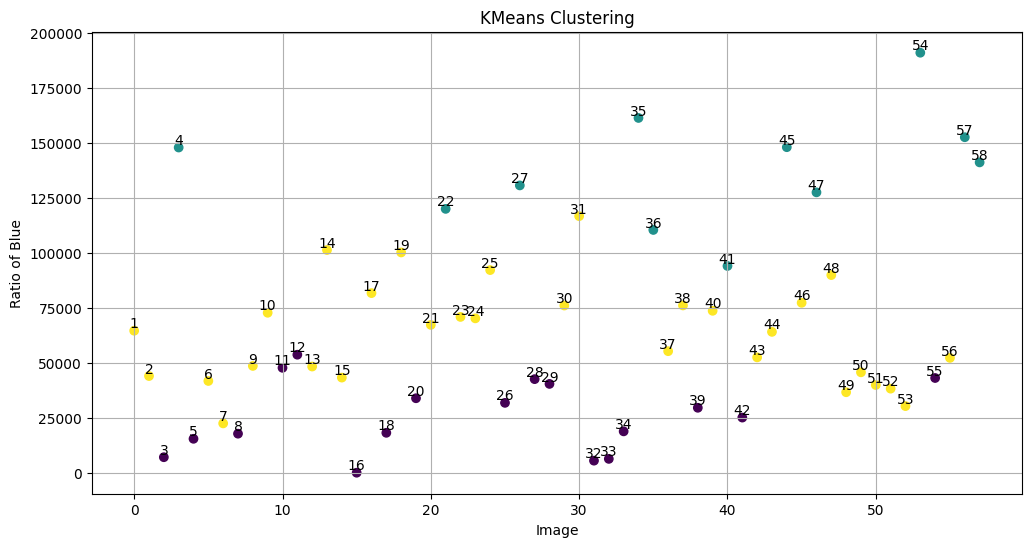
\includegraphics[width=1\linewidth]{Report/Images/ClusteringGroup.png}
    \caption{Clustering of the Embryos}
    \label{fig:KMeans_Clustering}
\end{figure}
\clearpage

\section*{Part 5.3 - Histogram of Oriented Gradients}
For this part, function \textit{hog} from library \textit{sklearn} was used. The data was consolidated into dataframes and split into 80-20 using $\text{train\_test\_split}$ function. \\Then, the model was trained on the training data, and the trained model was used to predict the test data. Using this, the accuracy was computed. 
\subsection*{Textures of the Parts of Embryo}
The texture was computed on the blue parts and the remaining parts of the embryo. 
The texture of the gene expression is tabulated in \ref{tab:texture_blue_0140} and \ref{tab:texture_blue_4158}. The texture of the remaining part is tabulated in \ref{tab:texture_yellow_0120} and \ref{tab:texture_yellow_2158}. 
\begin{table}[h!]
    \centering
    \begin{tabular}{|c|c|c|}
    \hline
    Image & Uniformity & Standard Deviation \\ \hline
    1 & 1 & 0.302619827 \\ \hline
    2 & 1 & 0.370923546 \\ \hline
    3 & 1 & 0.375136693 \\ \hline
    4 & 1 & 0.323010938 \\ \hline
    5 & 1 & 0.356169430 \\ \hline
    6 & 1 & 0.338897096 \\ \hline
    7 & 1 & 0.377314872 \\ \hline
    8 & 1 & 0.308471259 \\ \hline
    9 & 1 & 0.341413004 \\ \hline
    10 & 1 & 0.336791672 \\ \hline
    11 & 1 & 0.295951666 \\ \hline
    12 & 1 & 0.279088294 \\ \hline
    13 & 1 & 0.324691488 \\ \hline
    14 & 1 & 0.322645259 \\ \hline
    15 & 1 & 0.385790354 \\ \hline
    16 & 1 & 0.313925791 \\ \hline
    17 & 1 & 0.318236200 \\ \hline
    18 & 1 & 0.266986823 \\ \hline
    19 & 1 & 0.288487531 \\ \hline
    20 & 1 & 0.342248497 \\ \hline
    21 & 1 & 0.345044157 \\ \hline
    22 & 1 & 0.329015813 \\ \hline
    23 & 1 & 0.292647785 \\ \hline
    24 & 1 & 0.333544326 \\ \hline
    25 & 1 & 0.311267797 \\ \hline
    26 & 1 & 0.325018293 \\ \hline
    27 & 1 & 0.338373812 \\ \hline
    28 & 1 & 0.312860898 \\ \hline
    29 & 1 & 0.265757768 \\ \hline
    30 & 1 & 0.315485864 \\ \hline
    31 & 1 & 0.267096768 \\ \hline
    32 & 1 & 0.370674259 \\ \hline
    33 & 1 & 0.301985217 \\ \hline
    34 & 1 & 0.329807199 \\ \hline
    35 & 1 & 0.302917223 \\ \hline
    36 & 1 & 0.325402043 \\ \hline
    37 & 1 & 0.341098704 \\ \hline
    38 & 1 & 0.309894036 \\ \hline
    39 & 1 & 0.350465405 \\ \hline
    40 & 1 & 0.304783290 \\ \hline
    \end{tabular}
    \caption{Texture of the Blue Part of the Image - First 40 Images}
    \label{tab:texture_blue_0140}
\end{table}

\begin{table}[h!]
    \centering
    \begin{tabular}{|c|c|c|}
    \hline
    Image & Uniformity & Standard Deviation \\ \hline
    41 & 1 & 0.368317848 \\ \hline
    42 & 1 & 0.320139823 \\ \hline
    43 & 1 & 0.339564241 \\ \hline
    44 & 1 & 0.342528261 \\ \hline
    45 & 1 & 0.305189807 \\ \hline
    46 & 1 & 0.312129576 \\ \hline
    47 & 1 & 0.315755639 \\ \hline
    48 & 1 & 0.302413440 \\ \hline
    49 & 1 & 0.346705547 \\ \hline
    50 & 1 & 0.381467593 \\ \hline
    51 & 1 & 0.369497128 \\ \hline
    52 & 1 & 0.368913305 \\ \hline
    53 & 1 & 0.376186266 \\ \hline
    54 & 1 & 0.355141438 \\ \hline
    55 & 1 & 0.331788752 \\ \hline
    56 & 1 & 0.343655661 \\ \hline
    57 & 1 & 0.253546824 \\ \hline
    58 & 1 & 0.305536460 \\ \hline
    \end{tabular}
    \caption{Texture of the Blue Part of the Image - Last 20 Images (41 to 58)}
    \label{tab:texture_blue_4158}
\end{table}


\begin{table}[h!]
    \centering
    \begin{tabular}{|c|c|c|}
        \hline
        Image & Uniformity & Standard Deviation \\ \hline
        1 & 0.81684248 & 0.81684248 \\ \hline
        2 & 0.724831446 & 0.724831446 \\ \hline
        3 & 0.718544923 & 0.718544923 \\ \hline
        4 & 0.791327868 & 0.791327868 \\ \hline
        5 & 0.746286674 & 0.746286674 \\ \hline
        6 & 0.770297517 & 0.770297517 \\ \hline
        7 & 0.715266975 & 0.715266975 \\ \hline
        8 & 0.809690965 & 0.809690965 \\ \hline
        9 & 0.766874321 & 0.766874321 \\ \hline
        10 & 0.77314274 & 0.77314274 \\ \hline
        11 & 0.824825223 & 0.824825223 \\ \hline
        12 & 0.844219449 & 0.844219449 \\ \hline
        13 & 0.789150876 & 0.789150876 \\ \hline
        14 & 0.791800074 & 0.791800074 \\ \hline
        15 & 0.702331605 & 0.702331605 \\ \hline
        16 & 0.802901195 & 0.802901195 \\ \hline
        17 & 0.797451442 & 0.797451442 \\ \hline
        18 & 0.857436072 & 0.857436072 \\ \hline
        19 & 0.833549888 & 0.833549888 \\ \hline
        20 & 0.765731933 & 0.765731933 \\ \hline
    \end{tabular}
    \caption{Texture of the Remaining Part of the Image - First 20 Images}
    \label{tab:texture_yellow_0120}
\end{table}

\begin{table}[h!]
    \centering
    \begin{tabular}{|c|c|c|}
        \hline
        Image & Uniformity & Standard Deviation \\ \hline
        21 & 0.761889059 & 0.761889059 \\ \hline
        22 & 0.783497189 & 0.783497189 \\ \hline
        23 & 0.828714548 & 0.828714548 \\ \hline
        24 & 0.777496365 & 0.777496365 \\ \hline
        25 & 0.806224717 & 0.806224717 \\ \hline
        26 & 0.788726218 & 0.788726218 \\ \hline
        27 & 0.771006326 & 0.771006326 \\ \hline
        28 & 0.804236118 & 0.804236118 \\ \hline
        29 & 0.858745618 & 0.858745618 \\ \hline
        30 & 0.800937339 & 0.800937339 \\ \hline
        31 & 0.857318634 & 0.857318634 \\ \hline
        32 & 0.725201188 & 0.725201188 \\ \hline
        33 & 0.817609857 & 0.817609857 \\ \hline
        34 & 0.782454423 & 0.782454423 \\ \hline
        35 & 0.816482312 & 0.816482312 \\ \hline
        36 & 0.788227021 & 0.788227021 \\ \hline
        37 & 0.767303348 & 0.767303348 \\ \hline
        38 & 0.807931373 & 0.807931373 \\ \hline
        39 & 0.754348 & 0.754348 \\ \hline
        40 & 0.814214292 & 0.814214292 \\ \hline
        41 & 0.728683925 & 0.728683925 \\ \hline
        42 & 0.795020987 & 0.795020987 \\ \hline
        43 & 0.769392253 & 0.769392253 \\ \hline
        44 & 0.76534878 & 0.76534878 \\ \hline
        45 & 0.813718363 & 0.813718363 \\ \hline
        46 & 0.805150256 & 0.805150256 \\ \hline
        47 & 0.800596753 & 0.800596753 \\ \hline
        48 & 0.817092222 & 0.817092222 \\ \hline
        49 & 0.759590528 & 0.759590528 \\ \hline
        50 & 0.708964951 & 0.708964951 \\ \hline
        51 & 0.726943744 & 0.726943744 \\ \hline
        52 & 0.727805947 & 0.727805947 \\ \hline
        53 & 0.716967787 & 0.716967787 \\ \hline
        54 & 0.747749118 & 0.747749118 \\ \hline
        55 & 0.779832448 & 0.779832448 \\ \hline
        56 & 0.763801573 & 0.763801573 \\ \hline
        57 & 0.871428016 & 0.871428016 \\ \hline
        58 & 0.813294943 & 0.813294943 \\ \hline
    \end{tabular}
    \caption{Texture of the Remaining Part of the Images 21 - 58}
    \label{tab:texture_yellow_2158}
\end{table}
\clearpage
The results have been graphed out in figures \ref{fig:standard-hog} and \ref{fig:uniformity-hog}. Based on the figures, it is evident that the gene expression is homogeneous and uniform in texture, as the uniformity of this is 1. The remaining part of the embryo expresses variation in uniformity. This is also seen in the standard deviation values, as they are much lower, indicating less variability. 
\begin{figure}[h!]
    \centering
    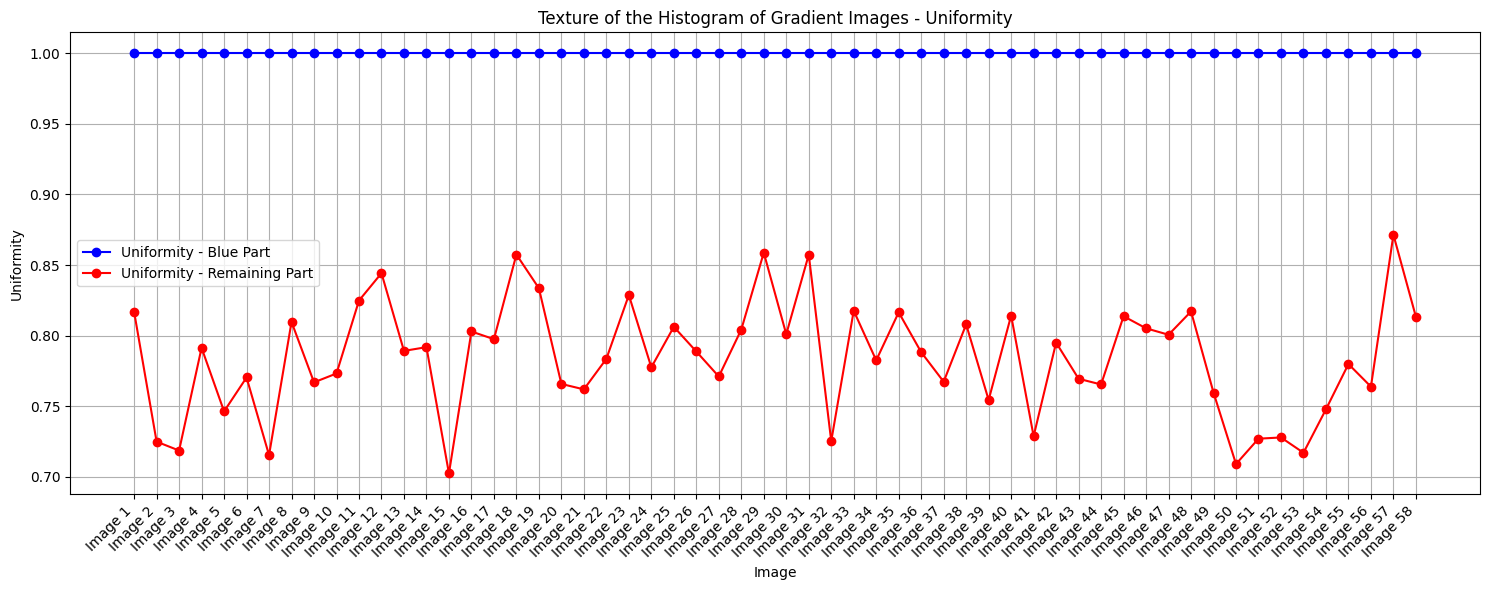
\includegraphics[width=0.75\linewidth]{Report/Images/HoG_Uniformity Graph.png}
    \caption{Texture - Uniformity of the Embryo}
    \label{fig:uniformity-hog}
\end{figure}

\begin{figure}[h!]
    \centering
    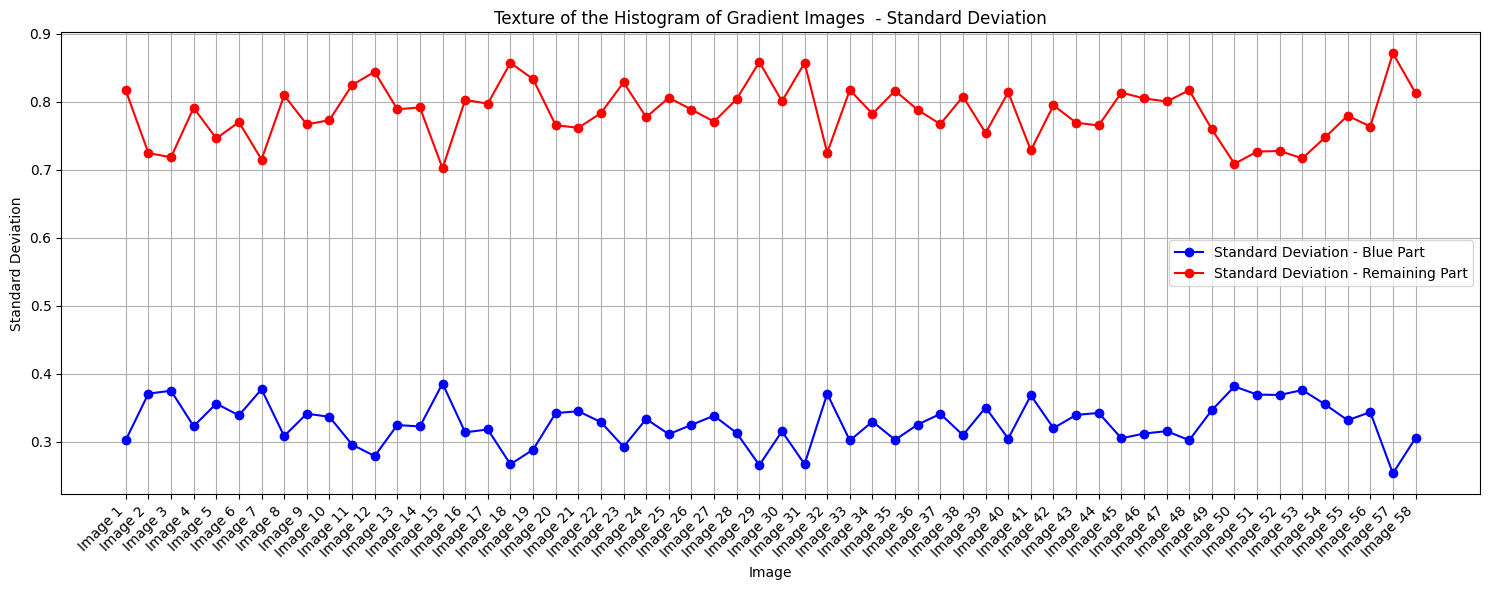
\includegraphics[width=0.75\linewidth]{Report/Images/HoG_StandardDeviation Graph.png}
    \caption{Texture - Standard Deviation of the Embryo}
    \label{fig:standard-hog}
\end{figure}
\subsection*{HoG - Variations in Cell Size}

Histogram of Gradients are computed using pixels per size. This is varied between (16,16) and (64,64). 
The HoG of the entire embryo with a pixel size of (16,16) is shown in figure  \ref{fig:hog_original_1616} and a pixel size of (64,64) is shown in figure \ref{fig:hog_original_6464}. \\ Similarly, a panel of the HoGs of the gene expression for pixel size (16,16) is shown in figure \ref{fig:hog_blue_1616}, and a pixel size of (64,64) is shown in figure \ref{fig:hog_blue_6464}. 
\begin{landscape}
    \begin{figure}
    \centering
    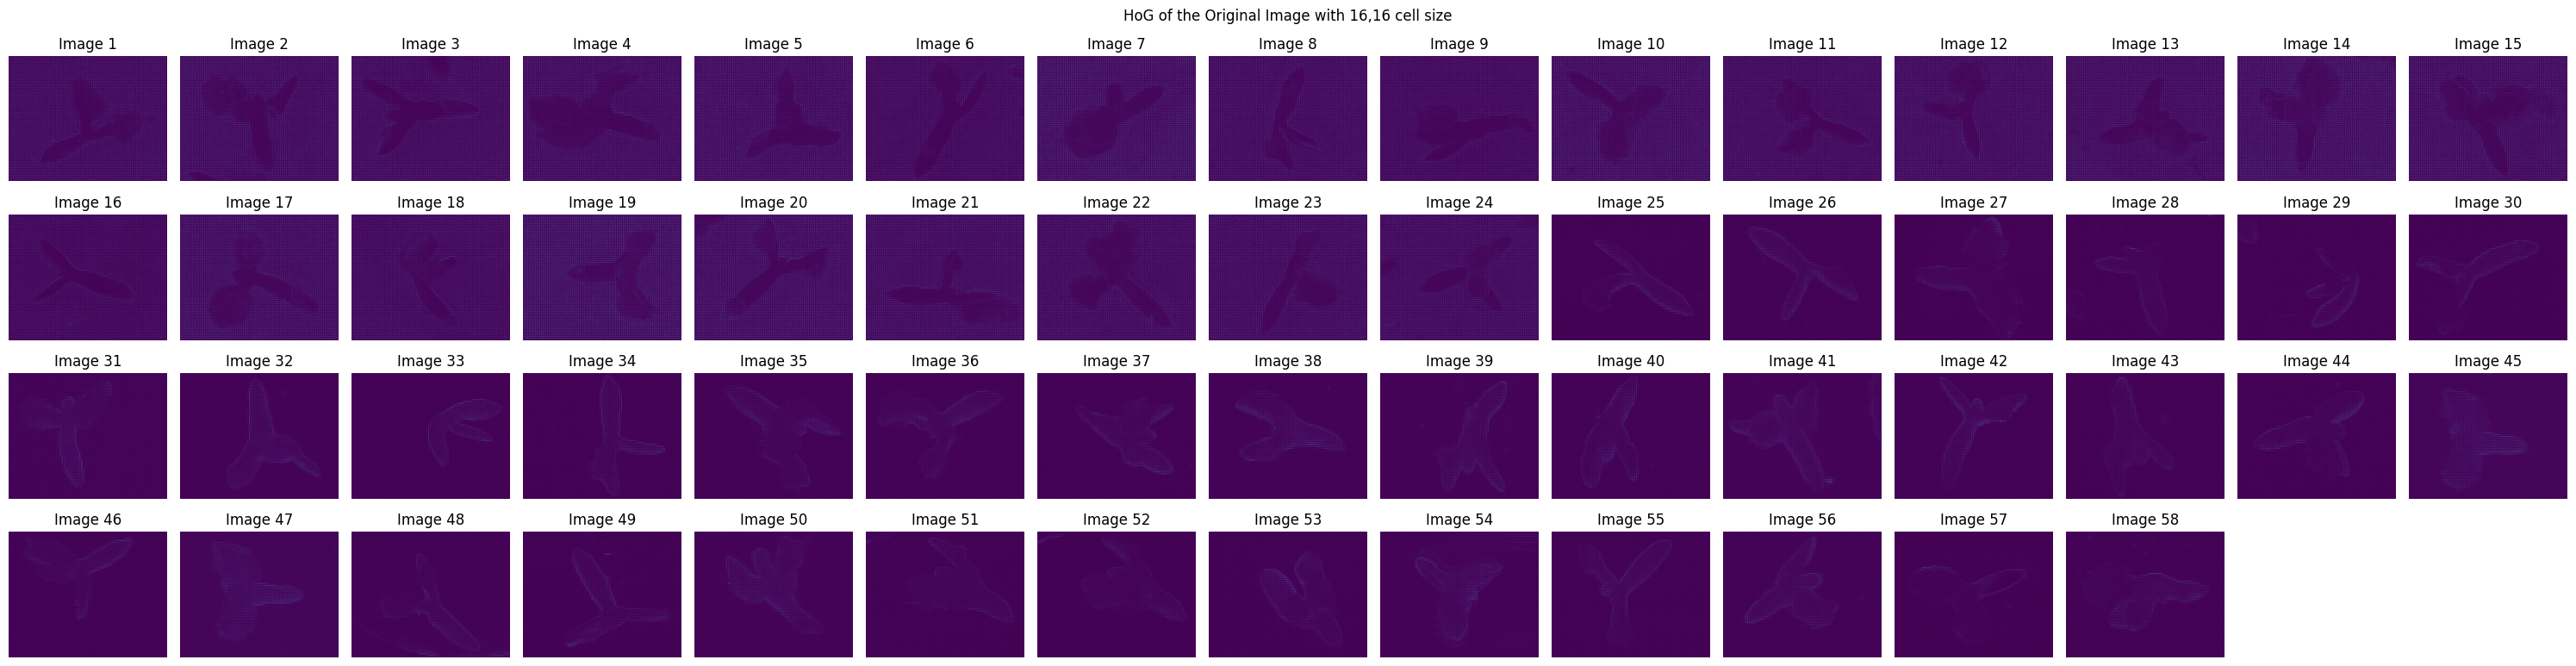
\includegraphics[width=1\linewidth, keepaspectratio]{Report/Images/Appendix Images/HoG/HoG_original_16,16.png}
    \caption{Histogram of the Entire Embryo with a pixel size of (16, 16)}
    \label{fig:hog_original_1616}
\end{figure}
\end{landscape}
\clearpage

\begin{landscape}
    \begin{figure}
    \centering
    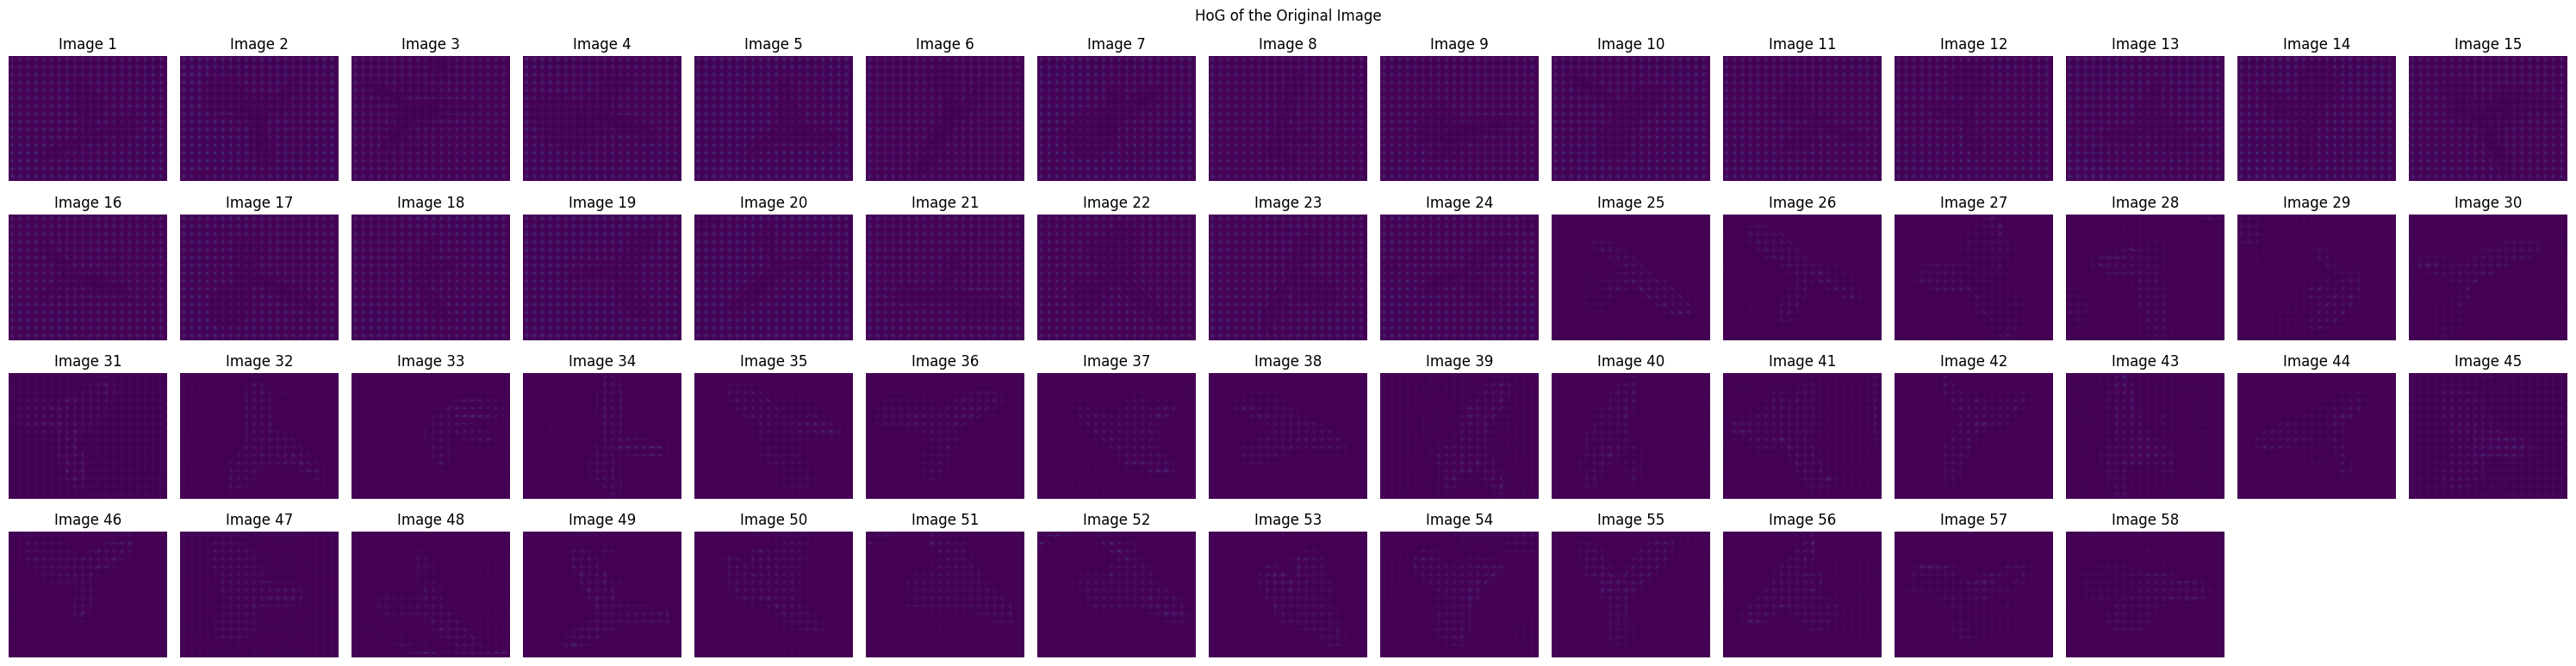
\includegraphics[width=1\linewidth, keepaspectratio]{Report/Images/Appendix Images/HoG/HoG_original_64,64.png}
    \caption{Histogram of the Entire Embryo with a pixel size of (64, 64)}
    \label{fig:hog_original_6464}
\end{figure}
\end{landscape}
\clearpage

\begin{landscape}
    \begin{figure}
    \centering
    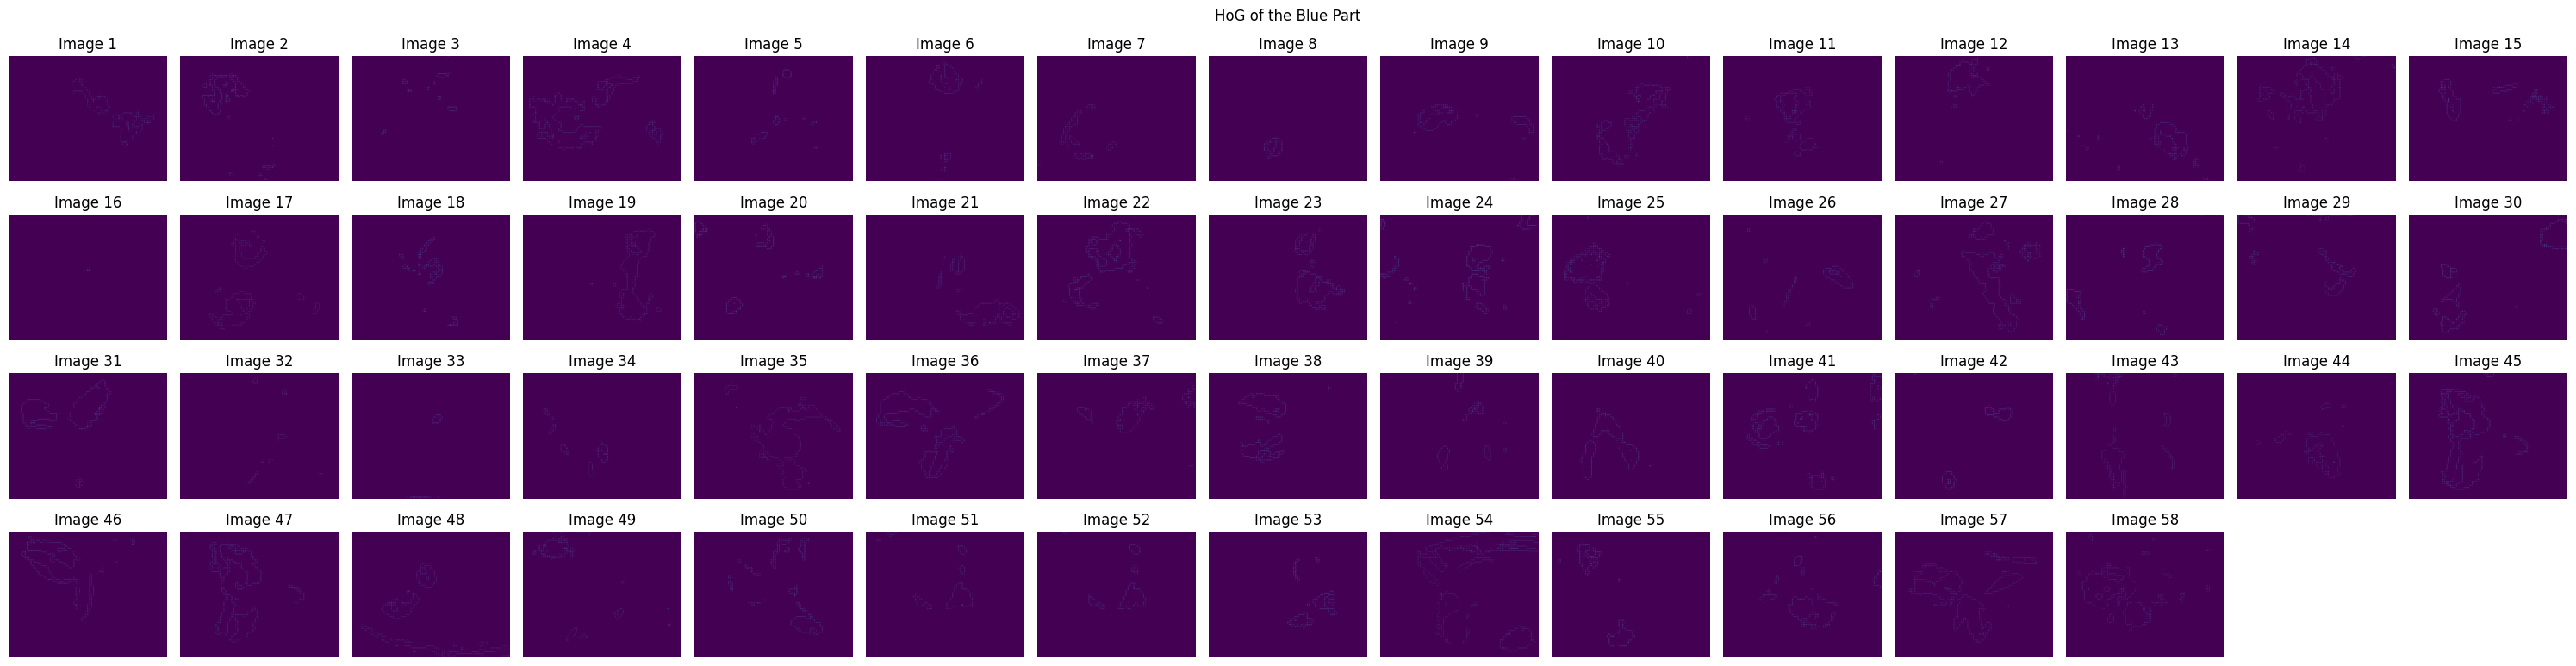
\includegraphics[width=1\linewidth, keepaspectratio]{Report/Images/Appendix Images/HoG/HoG_blue_16,16.png}
    \caption{Histogram of the Gene Expression (Blue Part) with a pixel size of (16, 16)}
    \label{fig:hog_blue_1616}
\end{figure}
\end{landscape}
\clearpage

\begin{landscape}
    \begin{figure}
    \centering
    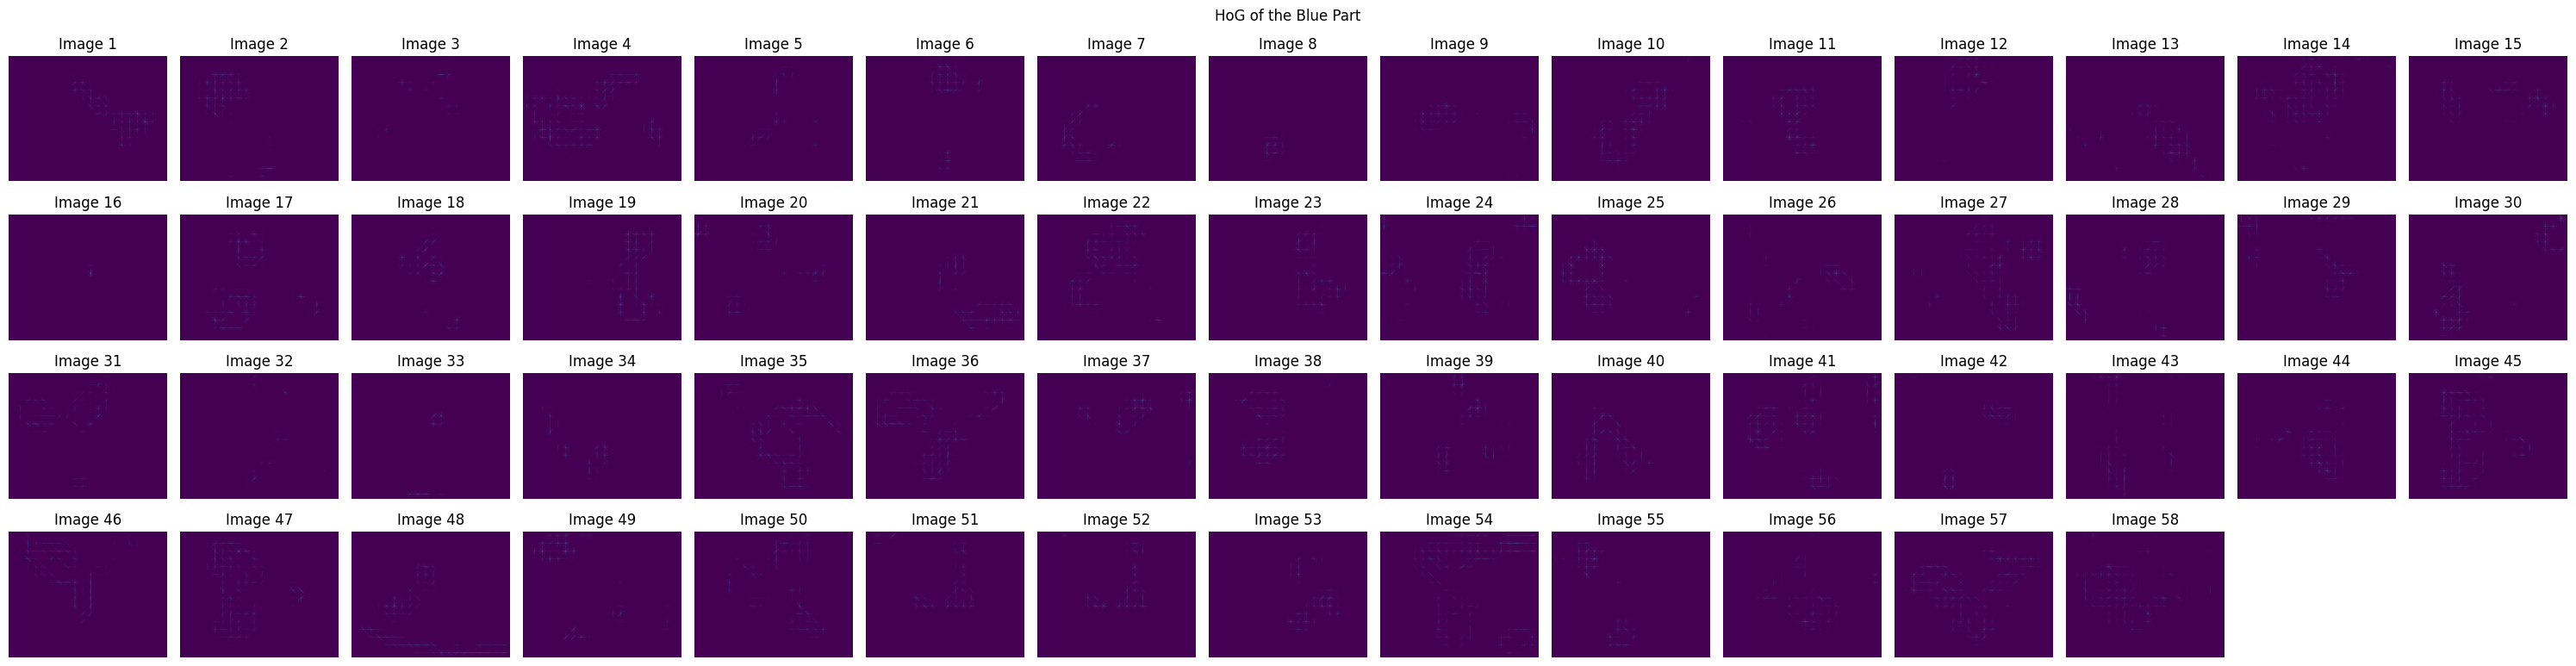
\includegraphics[width=1\linewidth, keepaspectratio]{Report/Images/Appendix Images/HoG/HoG_blue_64,64.png}
    \caption{Histogram of the Gene Expression (Blue Part) with a pixel size of (64, 64)}
    \label{fig:hog_blue_6464}
\end{figure}
\end{landscape}
\clearpage
\section*{Part 5.4 - SVM}
For this part, function \textit{SVM} from library \textit{sklearn} was used. The data was consolidated into dataframes and split into 80-20 using $\text{train\_test\_split}$ function. \\Then, the model was trained on the training data, and the trained model was used to predict the test data. Using this, the accuracy was computed. 
Initially, the data was sorted into three categories. The labels are from the clustering done initially, in figure  \ref{fig:KMeans_Clustering}
\subsection*{SVM on the HoG}
For this section, the HoG values generated from the previous section was used. The pixel size for this dataset is (16,16).
\begin{table}[h!]
    \centering
    \begin{tabular}{|p{0.3\linewidth} | p{0.6\linewidth}|}
    \hline
       Categories Used &  Size, SolidArea, Perimeter, Roundness, Solidity , Convexity , ConvexArea, ConvexPerimeter \\
    \hline
    \end{tabular}
    \label{tab:SVM_HoG}
\end{table}
When computed for the entire embryo, the accuracy was found to be 0.25
\subsection*{SVM on the Texture Dataset}
For this section, the texture values i.e., uniformity, standard deviation generated from the previous section was used. This was used on the blue part i.e, the gene expression and the remaining part of the embryo. 
\begin{table}[h!]
    \centering
    \begin{tabular}{|p{0.3\linewidth} | p{0.6\linewidth}|}
    \hline
       Categories Used &  Uniformity, Standard Deviation \\
    \hline
    \end{tabular}
    \label{tab:SVM_Texture}
\end{table}
When computed for the blue part of the embryo, the accuracy was found to be 0.5 and for the remaining part, the accuracy was 0.33. 
\subsection*{SVM on the Shape Dataset}
For this section, the shape values i.e., convexity, solidity generated from the previous section was used. This was used on the blue part i.e, the gene expression and the remaining part of the embryo. 
\begin{table}[h!]
    \centering
    \begin{tabular}{|p{0.3\linewidth} | p{0.6\linewidth}|}
    \hline
       Categories Used &  Convexity, Solidity \\
    \hline
    \end{tabular}
    \label{tab:Shape}
\end{table}
When computed for the blue part of the embryo, the accuracy was found to be 0.5 and for the remaining part, the accuracy was 0.33. 
\subsection*{SVM on the Combined Dataset}
For this section, the shape values i.e., convexity, solidity generated from the previous section was used. This was used on the blue part i.e, the gene expression and the remaining part of the embryo. 
\begin{table}[h!]
    \centering
    \begin{tabular}{|p{0.3\linewidth} | p{0.6\linewidth}|}
    \hline
       Categories Used &  Convexity, Solidity \\
    \hline
    \end{tabular}
    \label{tab:Shape}
\end{table}
When computed for the blue part of the embryo, the accuracy was found to be 0.5 and for the remaining part, the accuracy was 0.33. 
\subsection*{Quality of Separation in SVM Grouping}
\subsection*{Differences in Grouping}
\subsection*{Influence of Shape, Texture and HoG on the Classification}
While HoG focuses on capturing edge and gradient information within localized regions of an image, shape and texture provide valuable information on the nature of the object in the image. All three of them played a vital role in the classification models. 
\clearpage

\section*{Appendix} 
\subsection*{Segmentation based on Gene Expression} 
\label{sec:Segmentation}
The images were processed and segmented based on the gene expression (blue part) and the remaining part. 
\begin{figure}[h!]
\centering
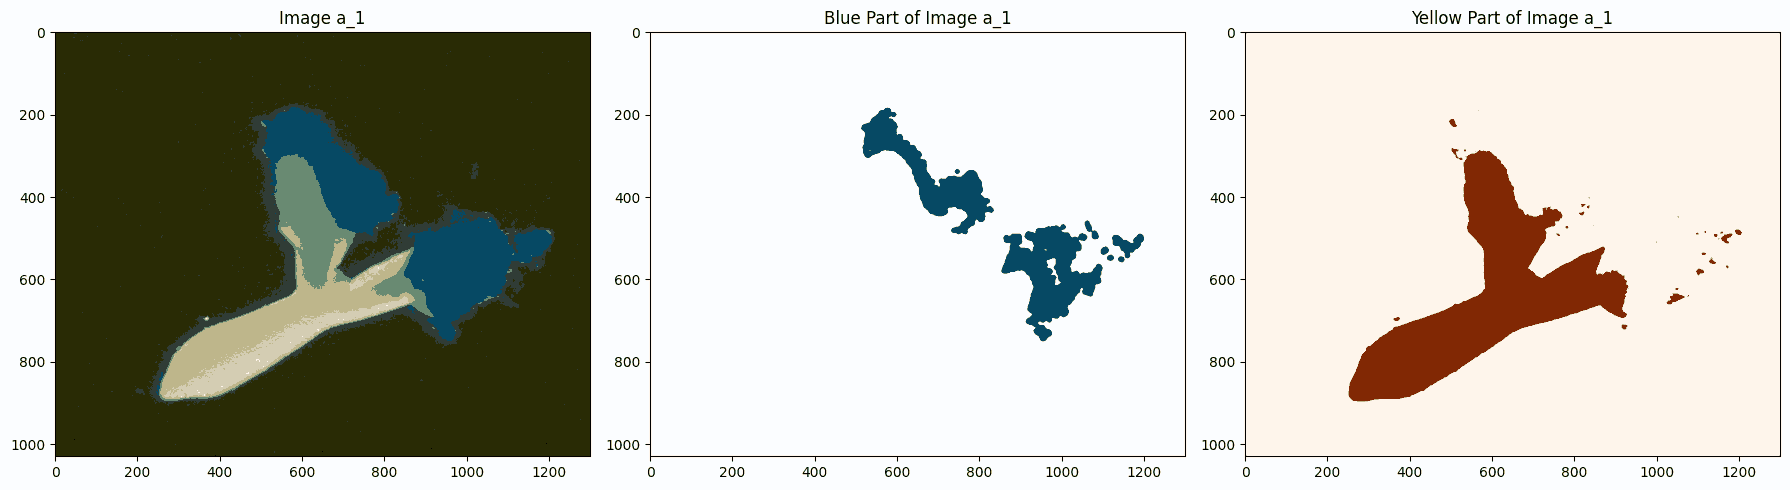
\includegraphics[width=0.95\textwidth]{Report/Images/Appendix Images/ColorSegments/Image1.png}
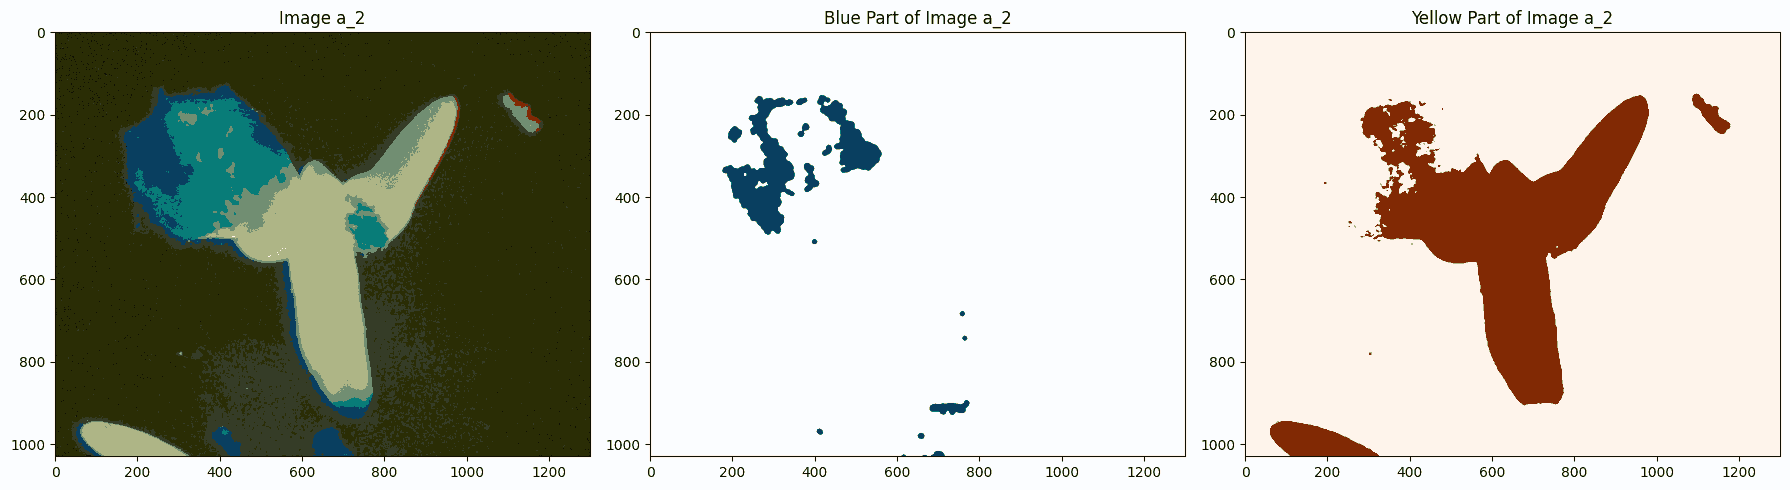
\includegraphics[width=0.95\textwidth]{Report/Images/Appendix Images/ColorSegments/Image2.png}
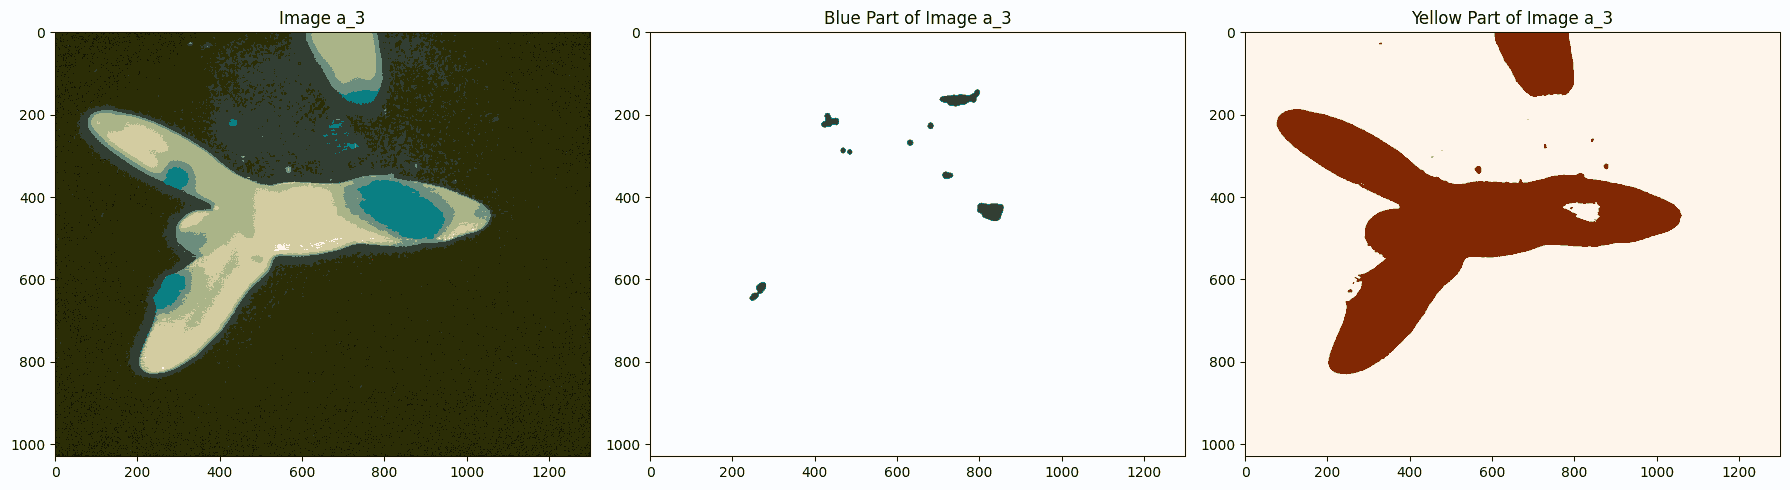
\includegraphics[width=0.95\textwidth]{Report/Images/Appendix Images/ColorSegments/Image3.png}
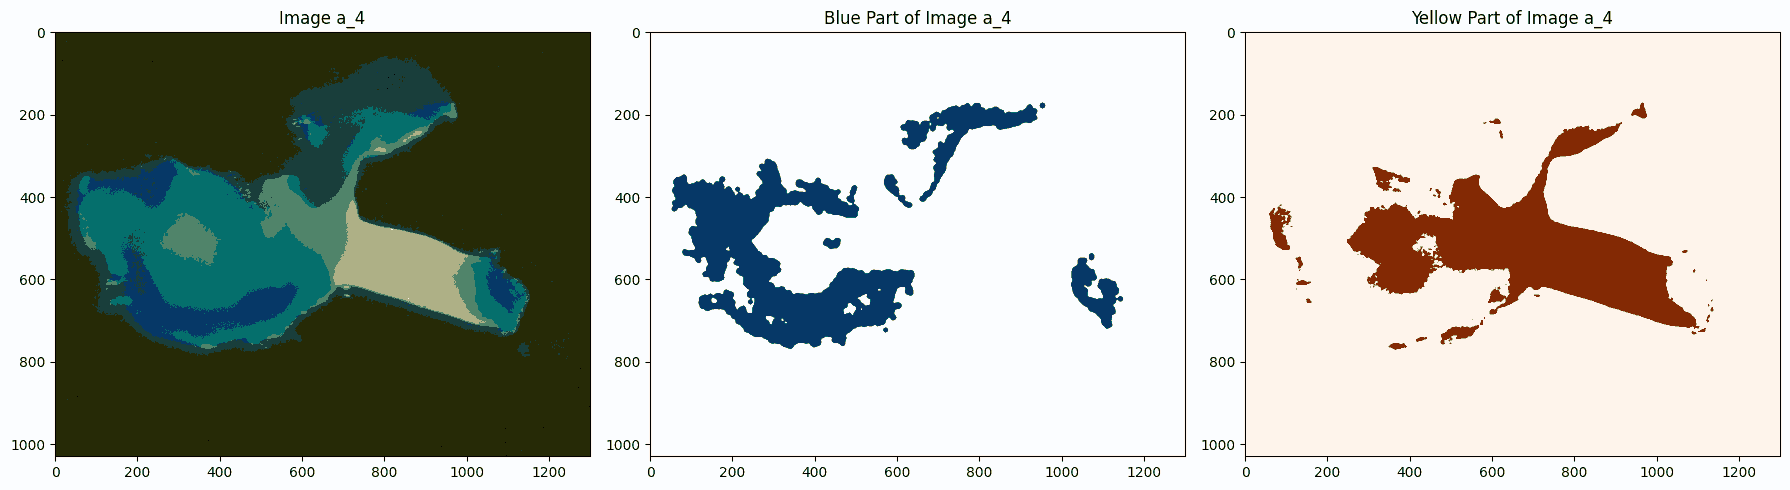
\includegraphics[width=0.95\textwidth]{Report/Images/Appendix Images/ColorSegments/Image4.png}
\caption{The series of segmented images (blue and yellow part) for the images 1-4} 
\label{fig:segment1-4}
\end{figure}
\begin{figure}[h!]
\centering
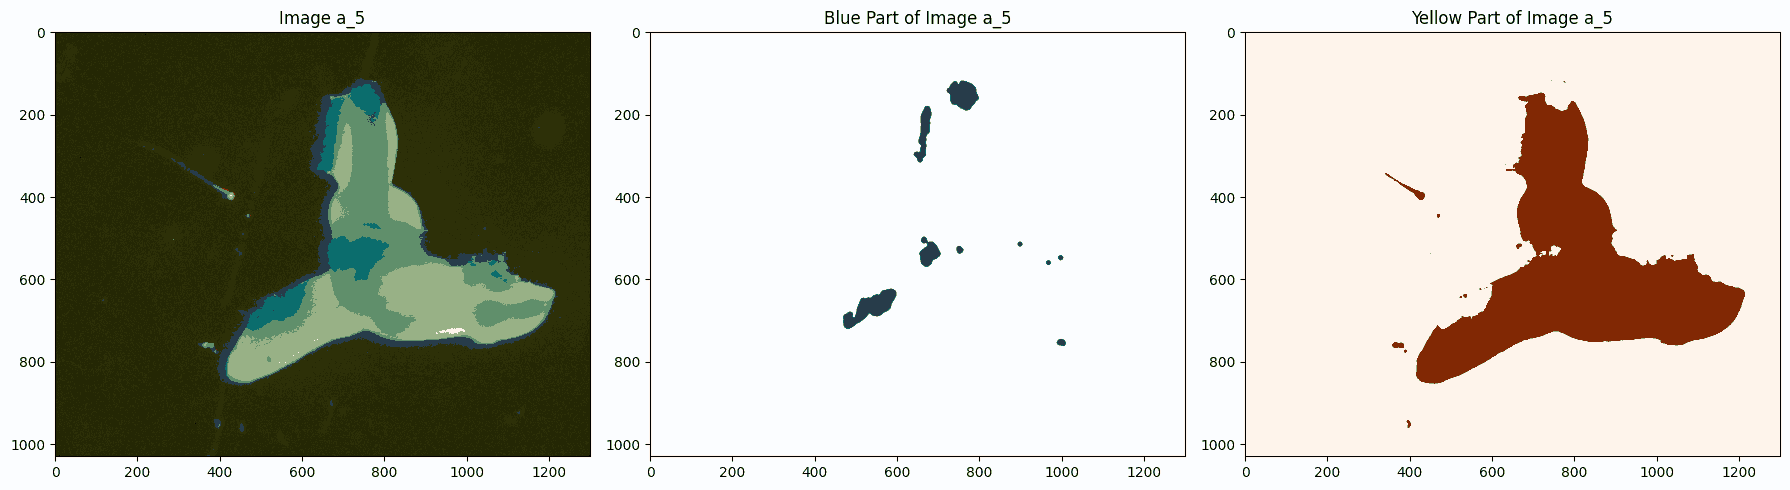
\includegraphics[width=0.95\textwidth]{Report/Images/Appendix Images/ColorSegments/Image5.png}
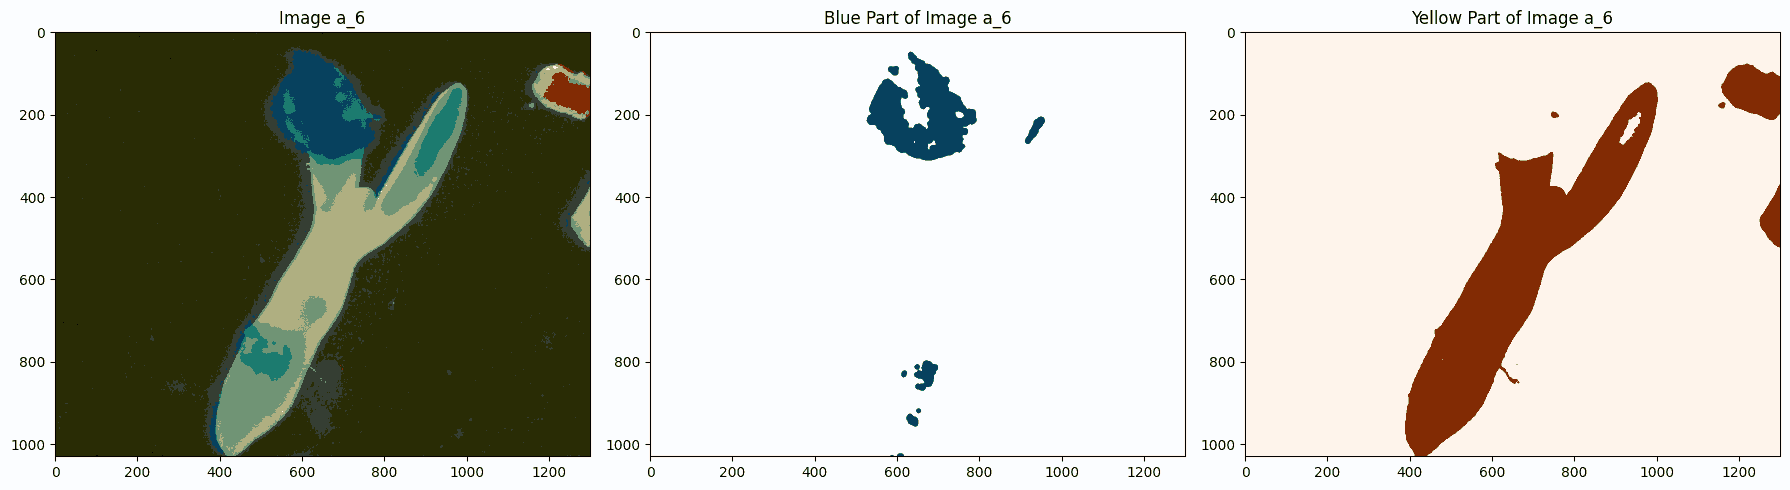
\includegraphics[width=0.95\textwidth]{Report/Images/Appendix Images/ColorSegments/Image6.png}
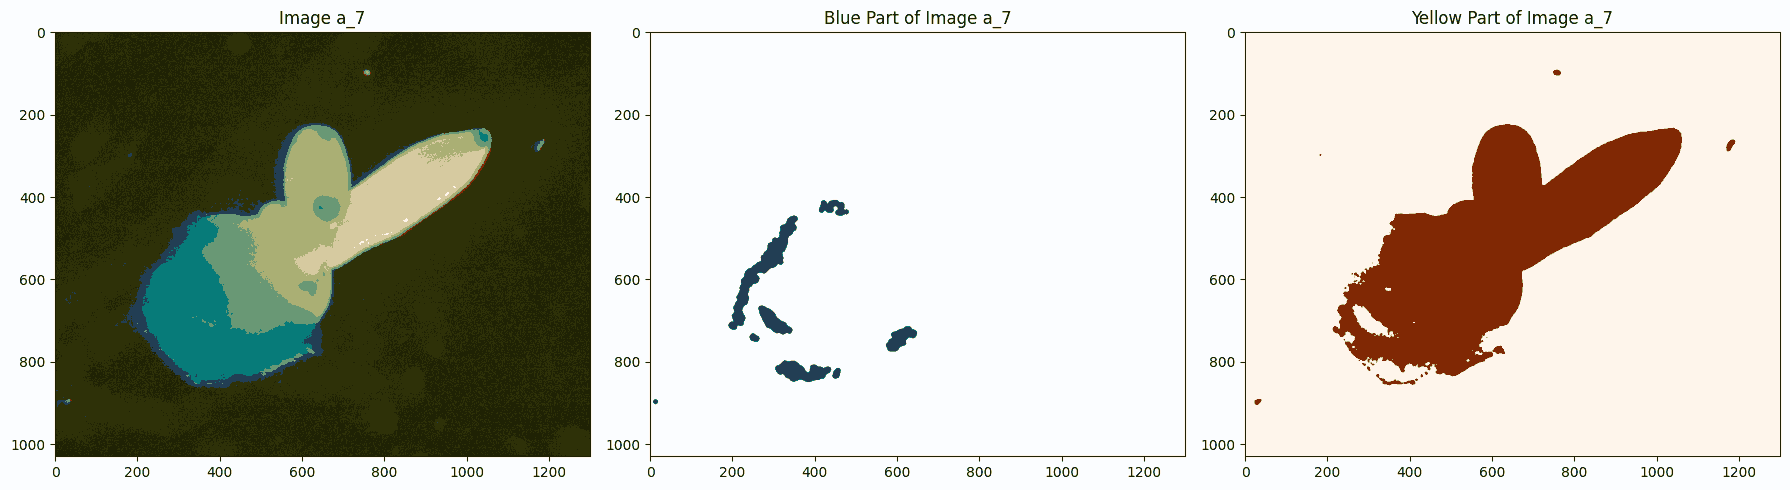
\includegraphics[width=0.95\textwidth]{Report/Images/Appendix Images/ColorSegments/Image7.png}
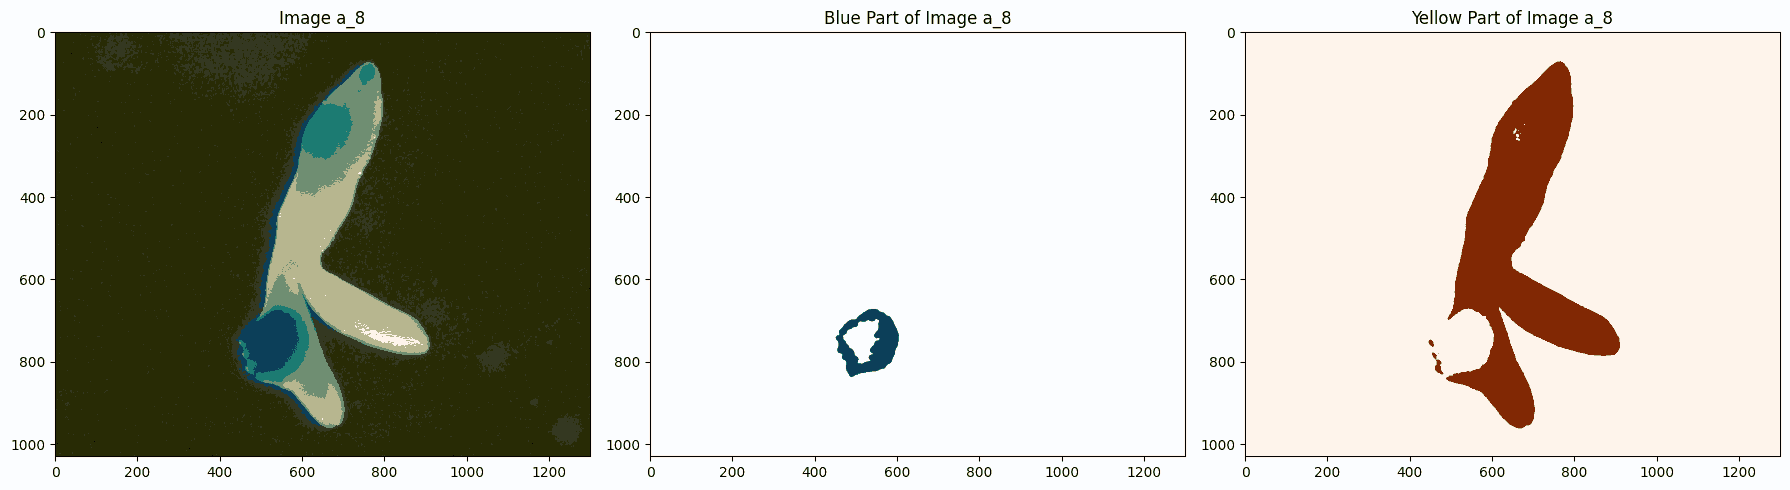
\includegraphics[width=0.95\textwidth]{Report/Images/Appendix Images/ColorSegments/Image8.png}
\caption{The series of segmented images (blue and yellow part) for the images 5-8} 
\label{fig:segment5-8}
\end{figure}
\begin{figure}[h!]
\centering
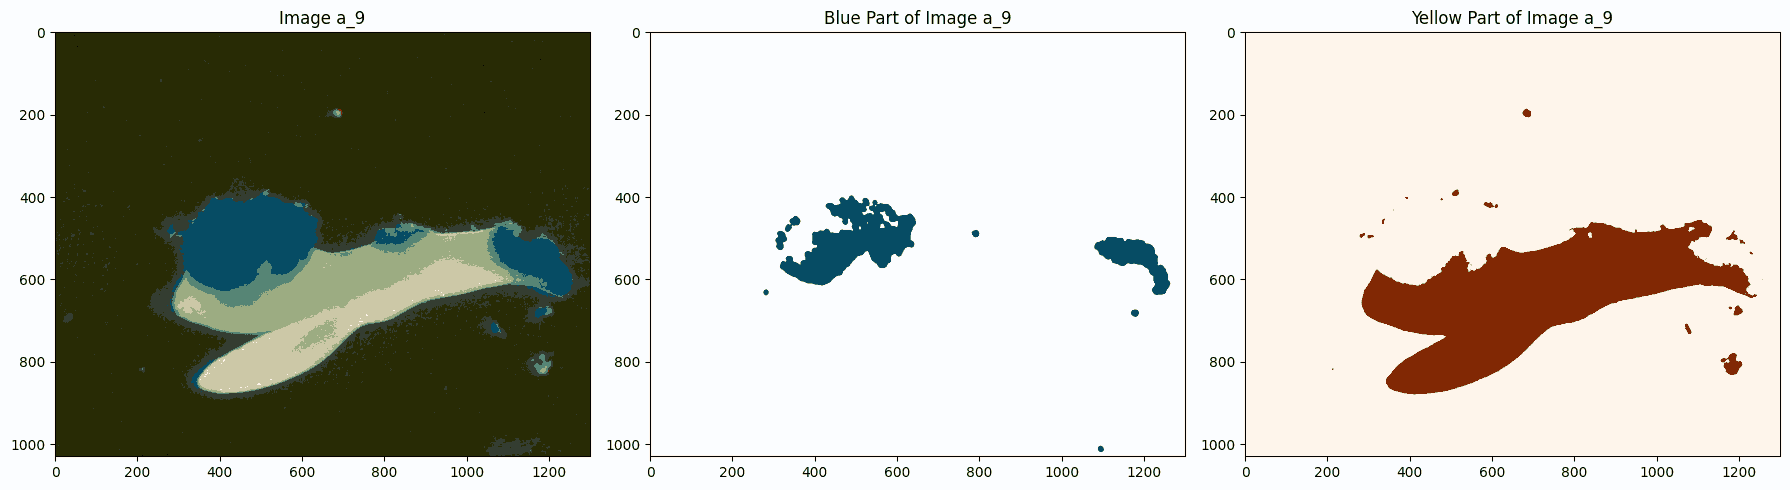
\includegraphics[width=0.95\textwidth]{Report/Images/Appendix Images/ColorSegments/Image9.png}
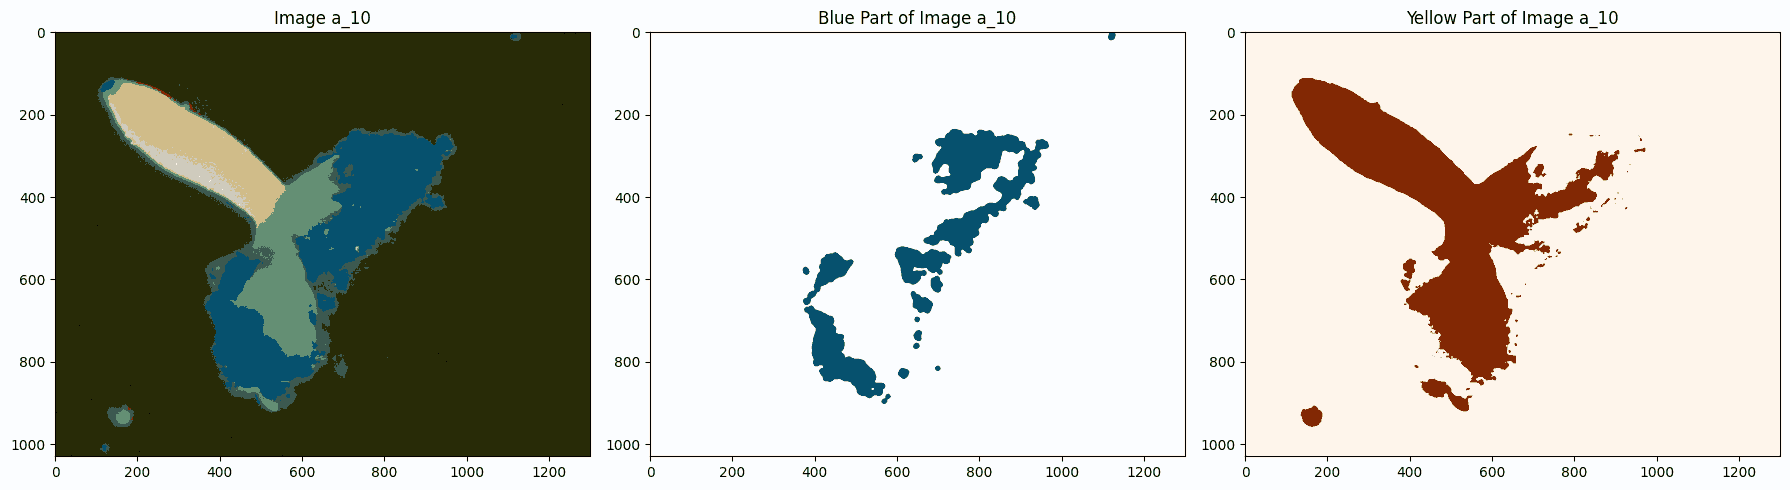
\includegraphics[width=0.95\textwidth]{Report/Images/Appendix Images/ColorSegments/Image10.png}
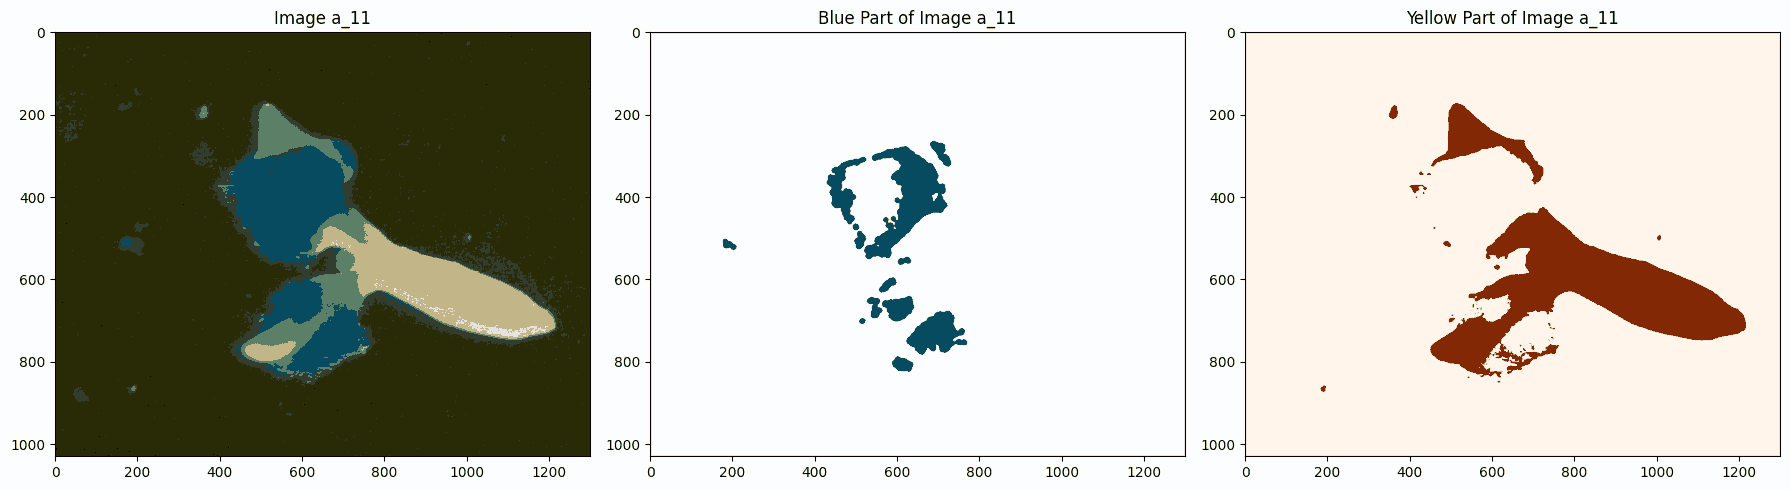
\includegraphics[width=0.95\textwidth]{Report/Images/Appendix Images/ColorSegments/Image11.png}
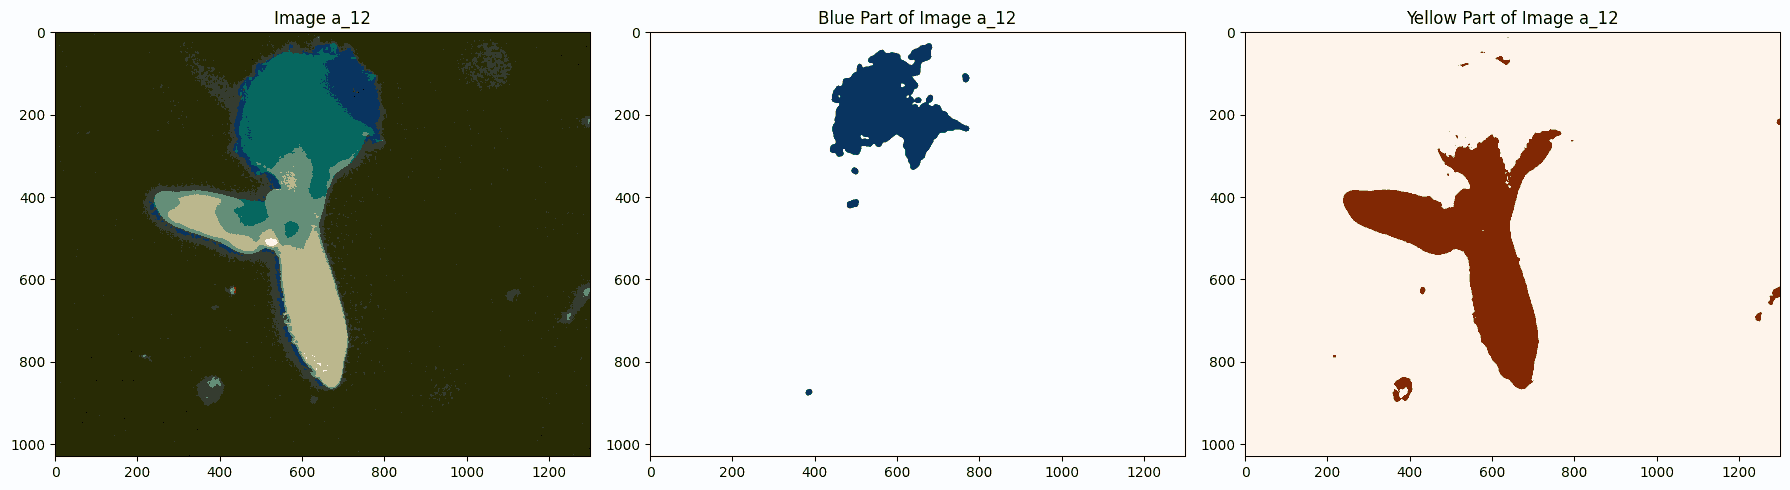
\includegraphics[width=0.95\textwidth]{Report/Images/Appendix Images/ColorSegments/Image12.png}
\caption{The series of segmented images (blue and yellow part) for the images 9-12} 
\label{fig:segment9-12}
\end{figure}

\begin{figure}[h!]
\centering
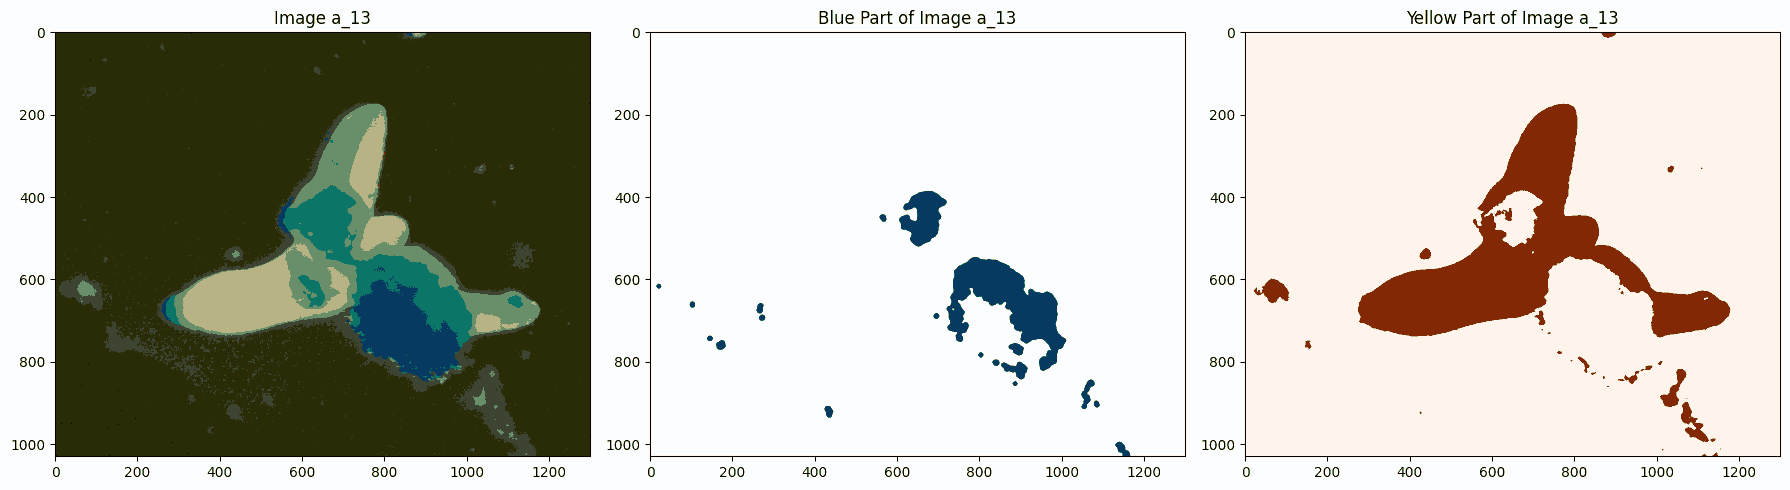
\includegraphics[width=0.95\textwidth]{Report/Images/Appendix Images/ColorSegments/Image13.png}
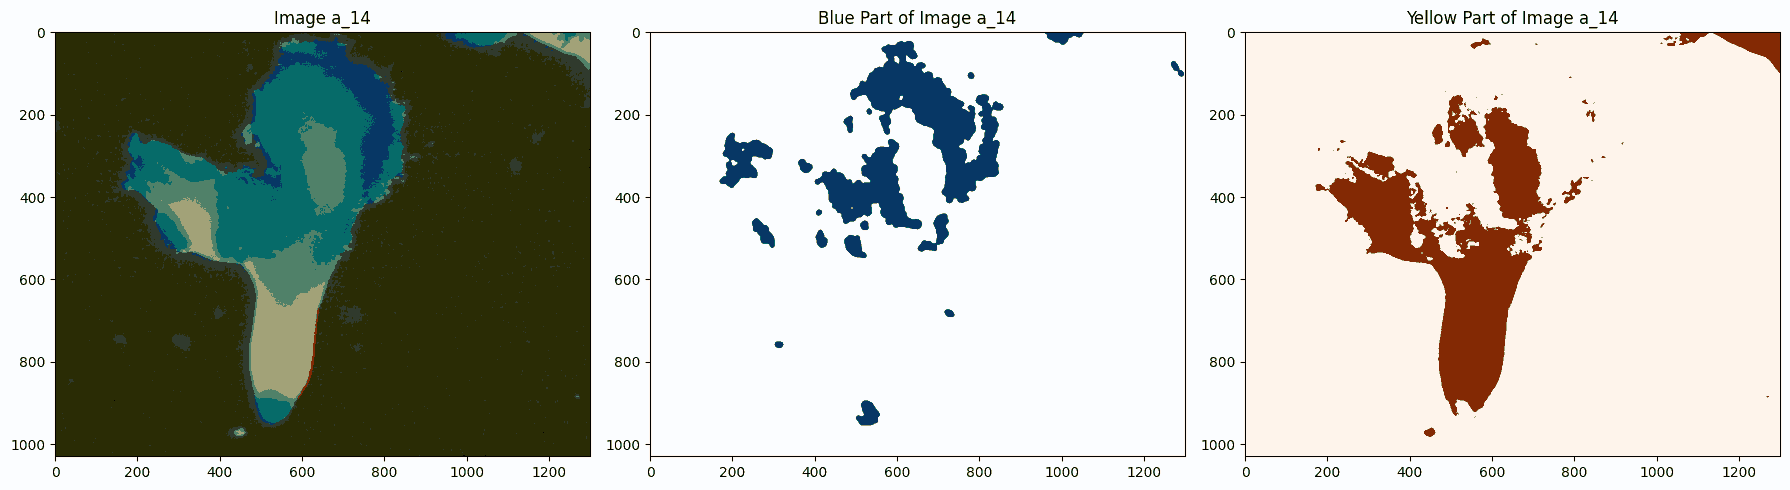
\includegraphics[width=0.95\textwidth]{Report/Images/Appendix Images/ColorSegments/Image14.png}
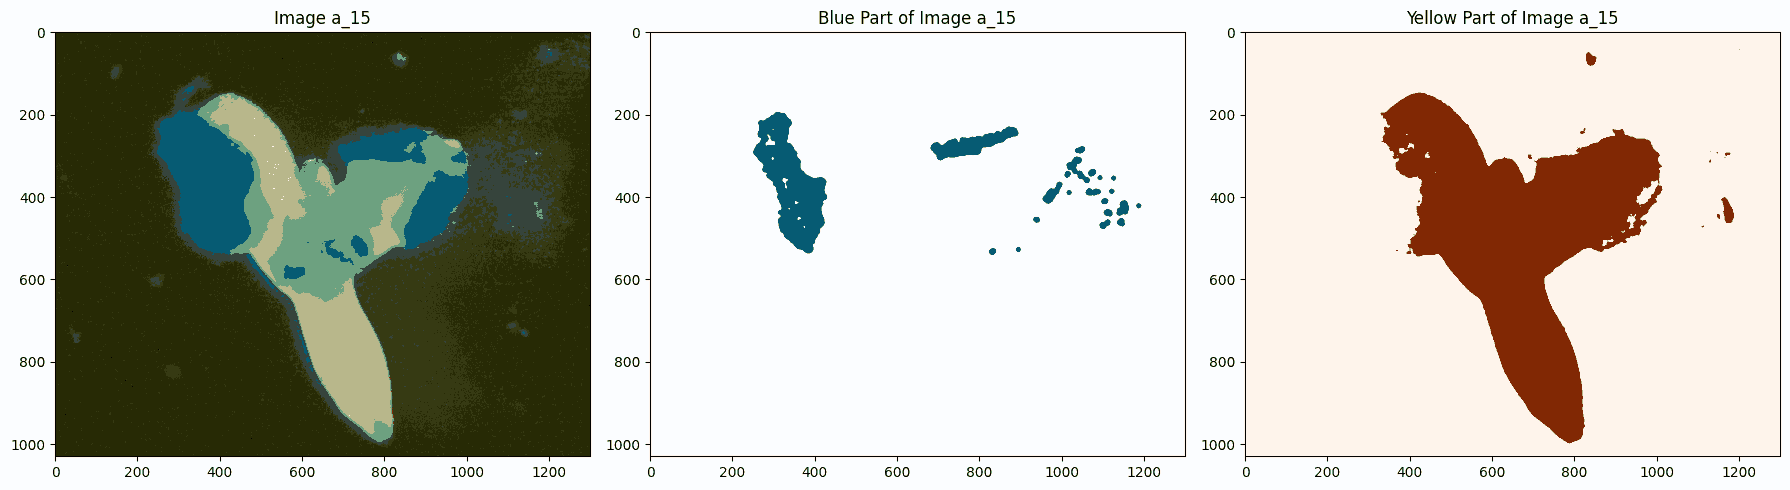
\includegraphics[width=0.95\textwidth]{Report/Images/Appendix Images/ColorSegments/Image15.png}
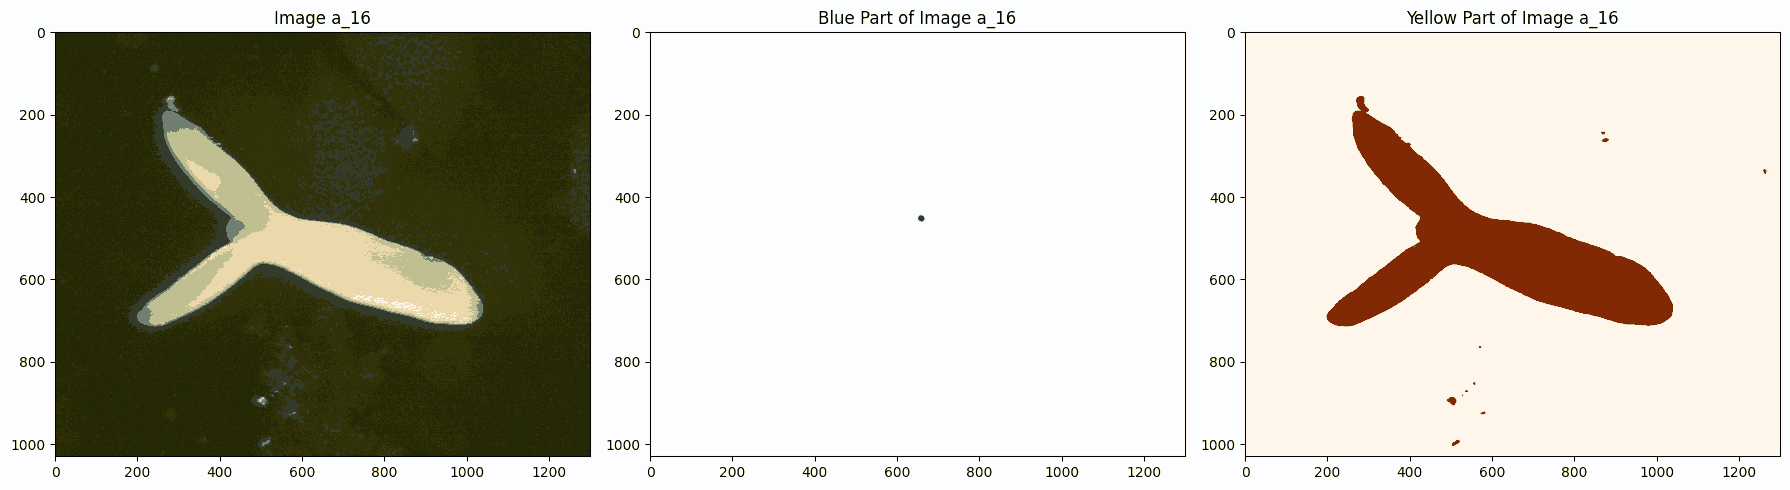
\includegraphics[width=0.95\textwidth]{Report/Images/Appendix Images/ColorSegments/Image16.png}
\caption{The series of segmented images (blue and yellow part) for the images 13-16} 
\label{fig:segment13-16}
\end{figure}
\begin{figure}[h!]
\centering
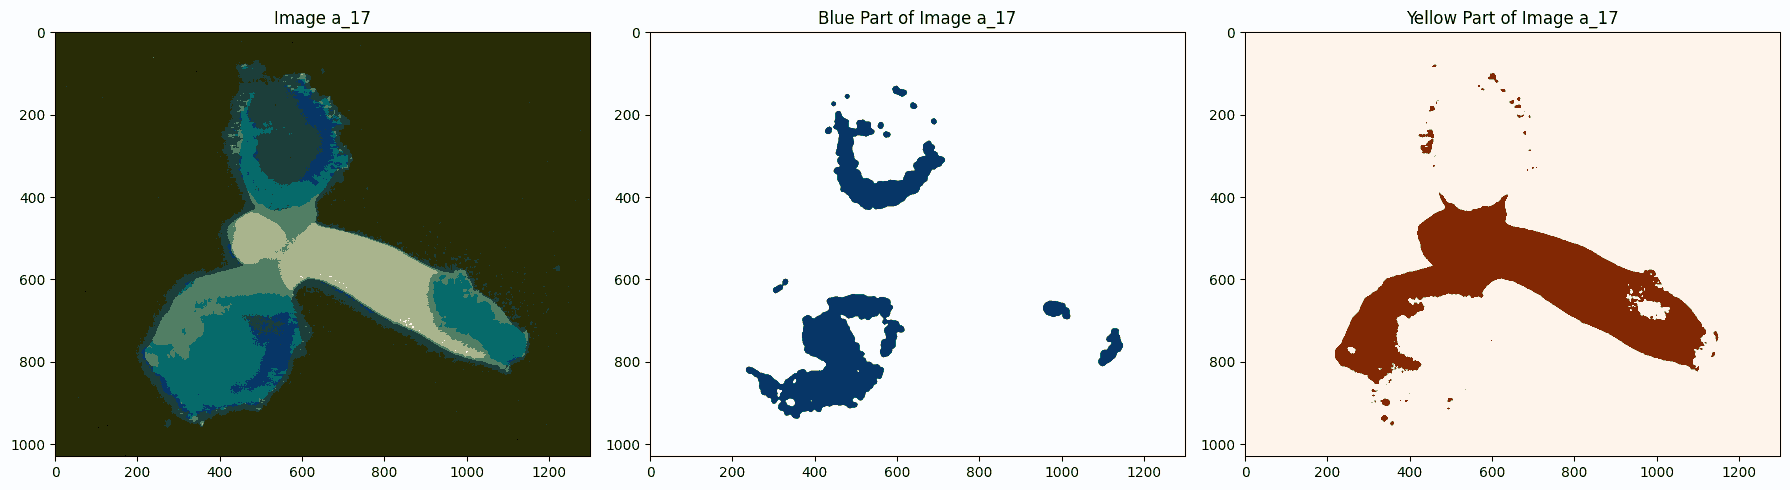
\includegraphics[width=0.95\textwidth]{Report/Images/Appendix Images/ColorSegments/Image17.png}
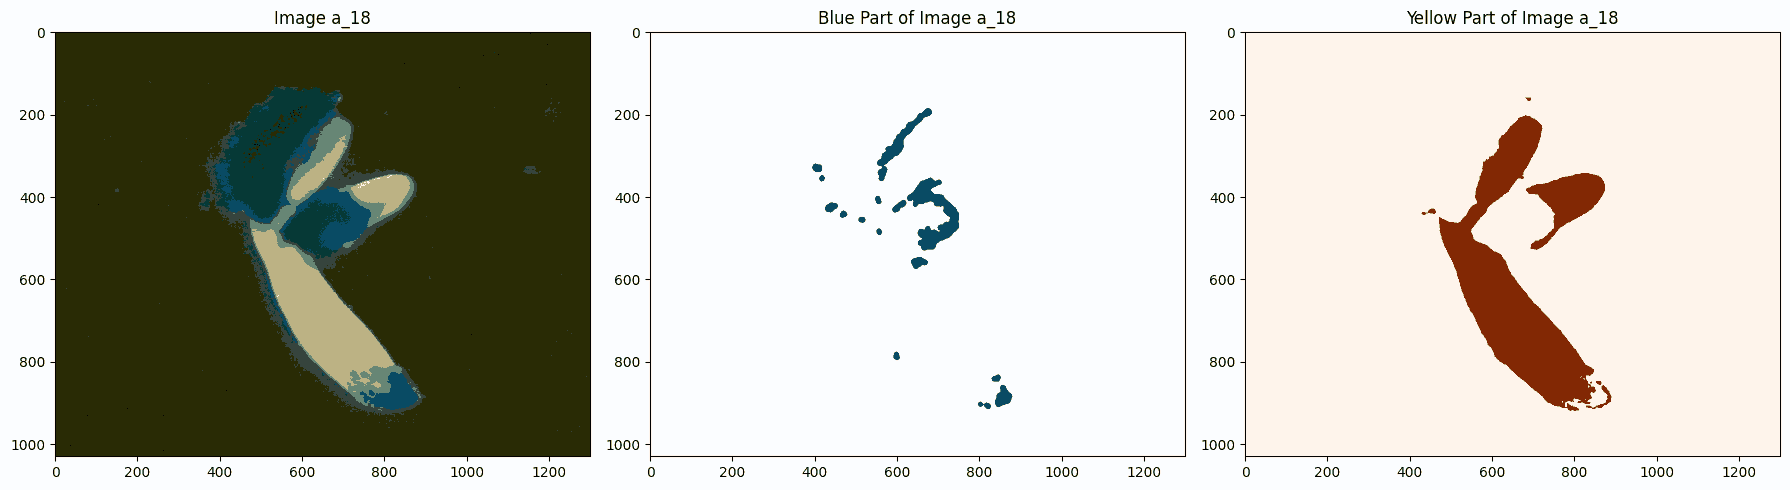
\includegraphics[width=0.95\textwidth]{Report/Images/Appendix Images/ColorSegments/Image18.png}
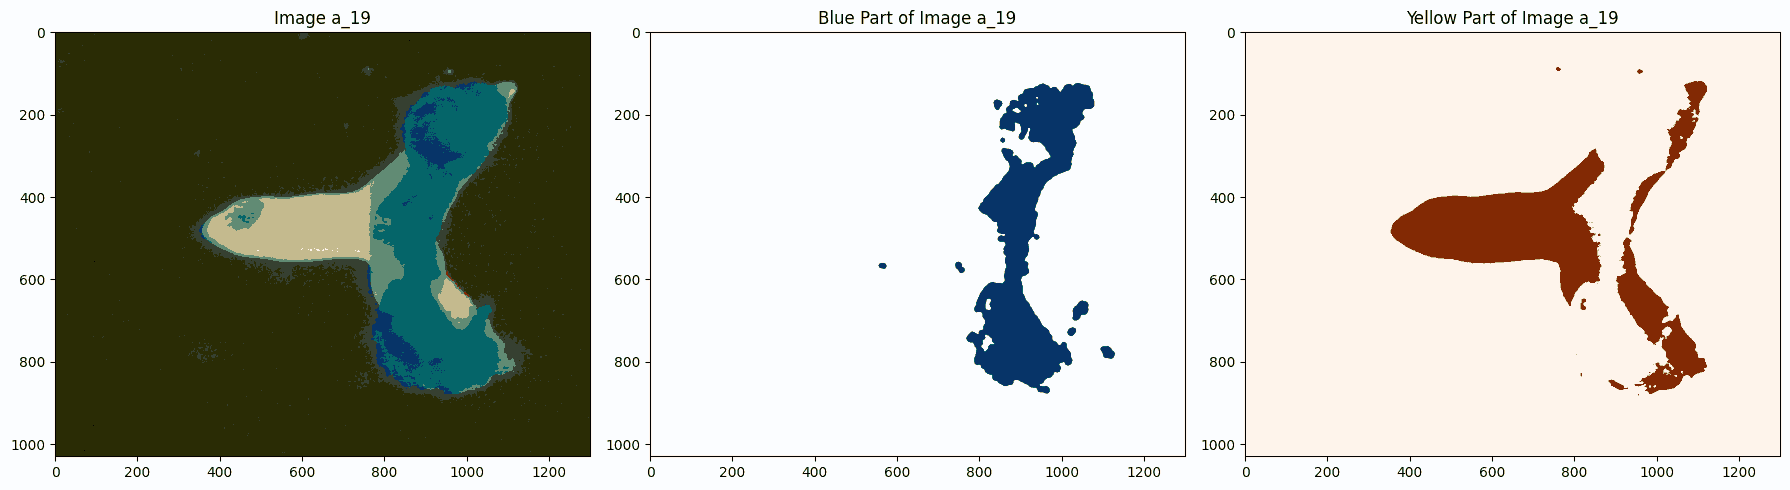
\includegraphics[width=0.95\textwidth]{Report/Images/Appendix Images/ColorSegments/Image19.png}
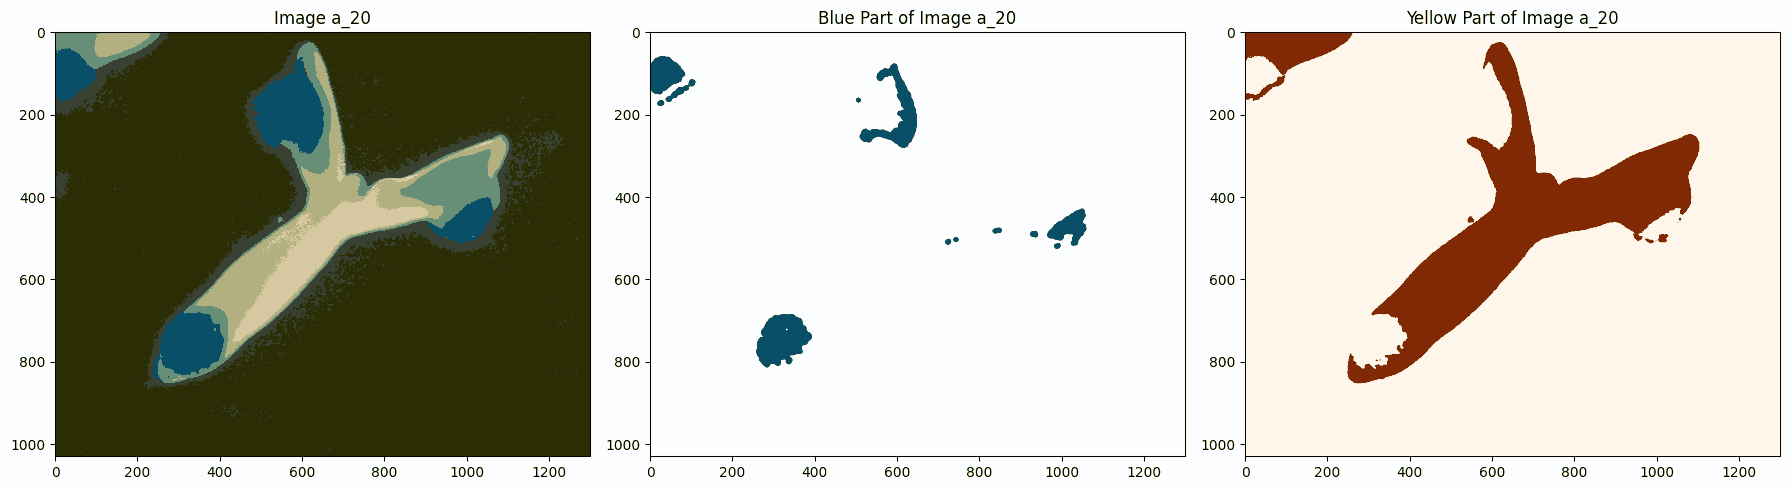
\includegraphics[width=0.95\textwidth]{Report/Images/Appendix Images/ColorSegments/Image20.png}
\caption{The series of segmented images (blue and yellow part) for the images 17-20} 
\label{fig:segment17-20}
\end{figure}
\begin{figure}[h!]
\centering
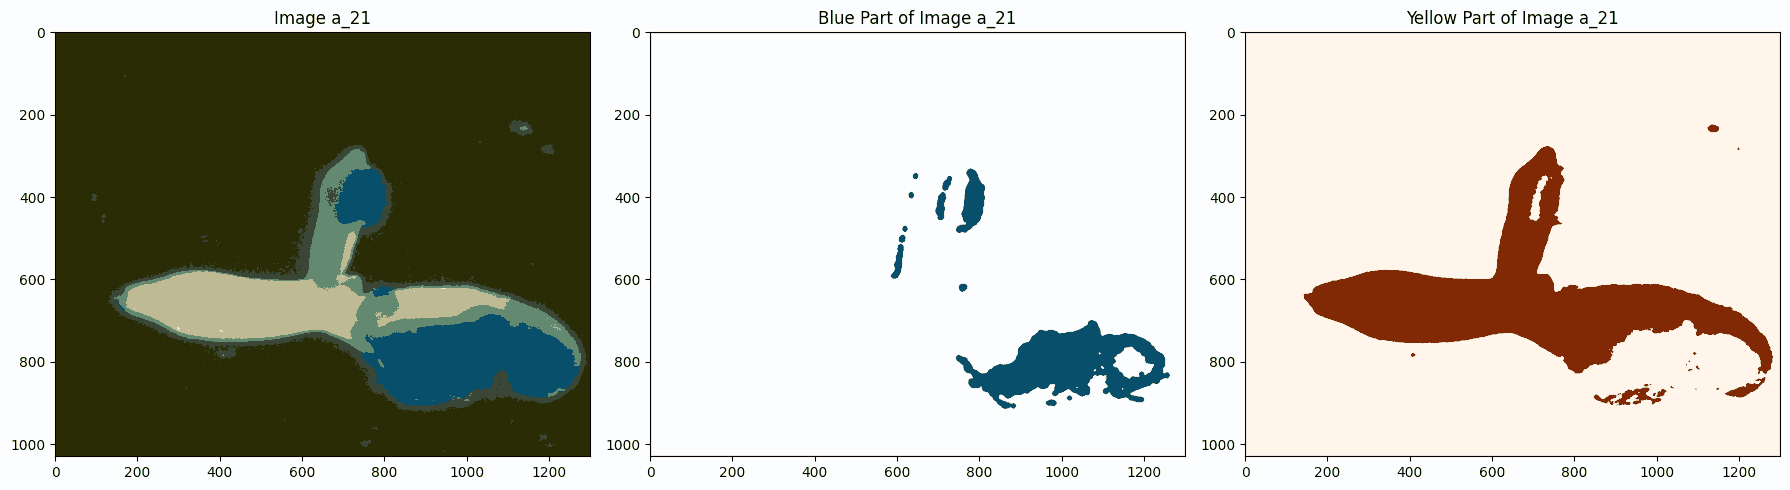
\includegraphics[width=0.95\textwidth]{Report/Images/Appendix Images/ColorSegments/Image21.png}
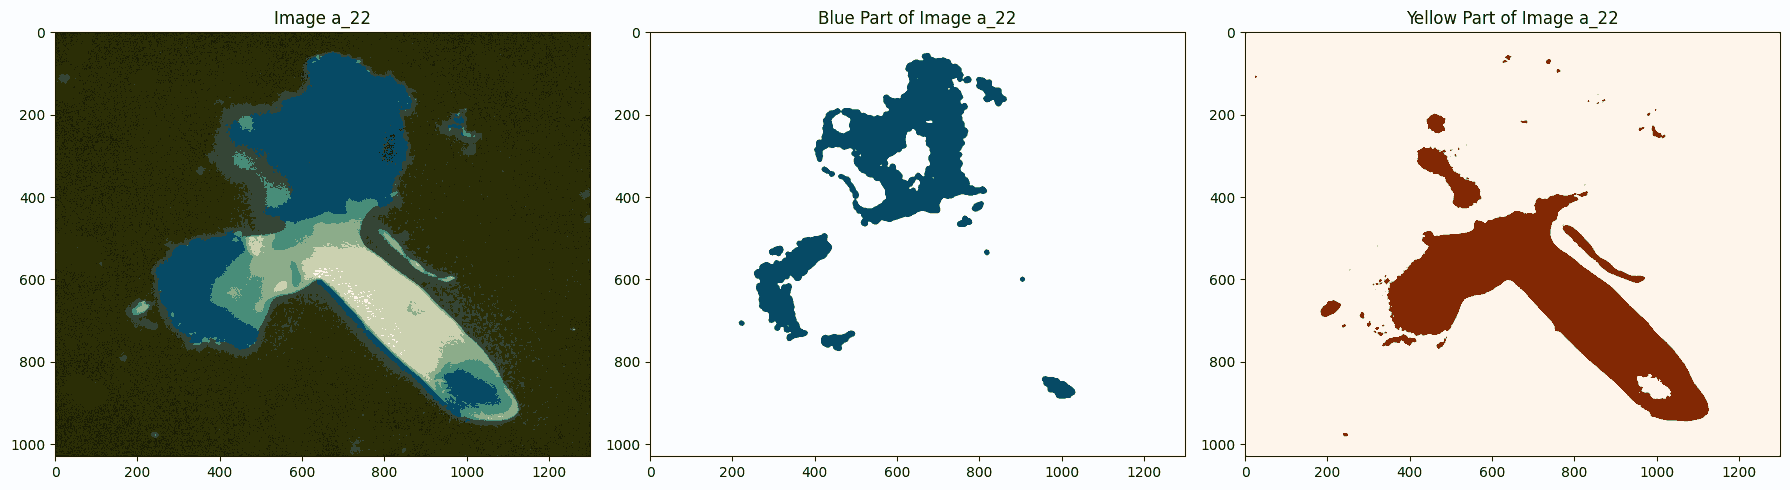
\includegraphics[width=0.95\textwidth]{Report/Images/Appendix Images/ColorSegments/Image22.png}
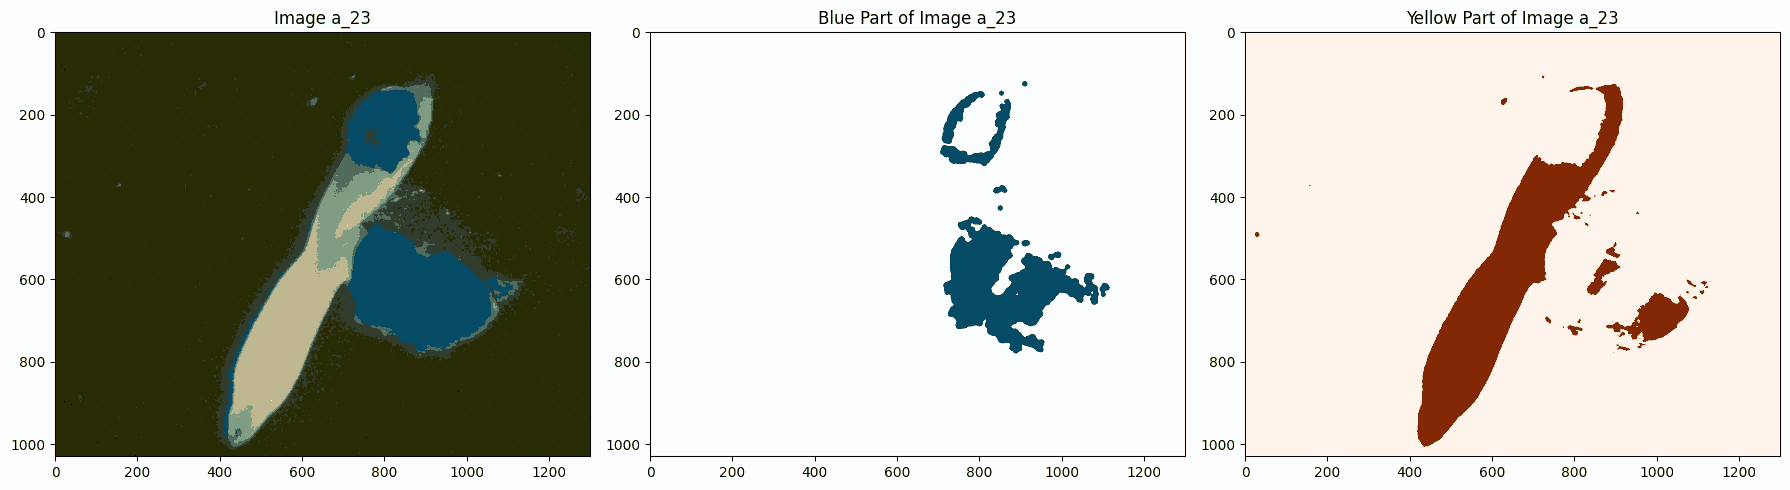
\includegraphics[width=0.95\textwidth]{Report/Images/Appendix Images/ColorSegments/Image23.png}
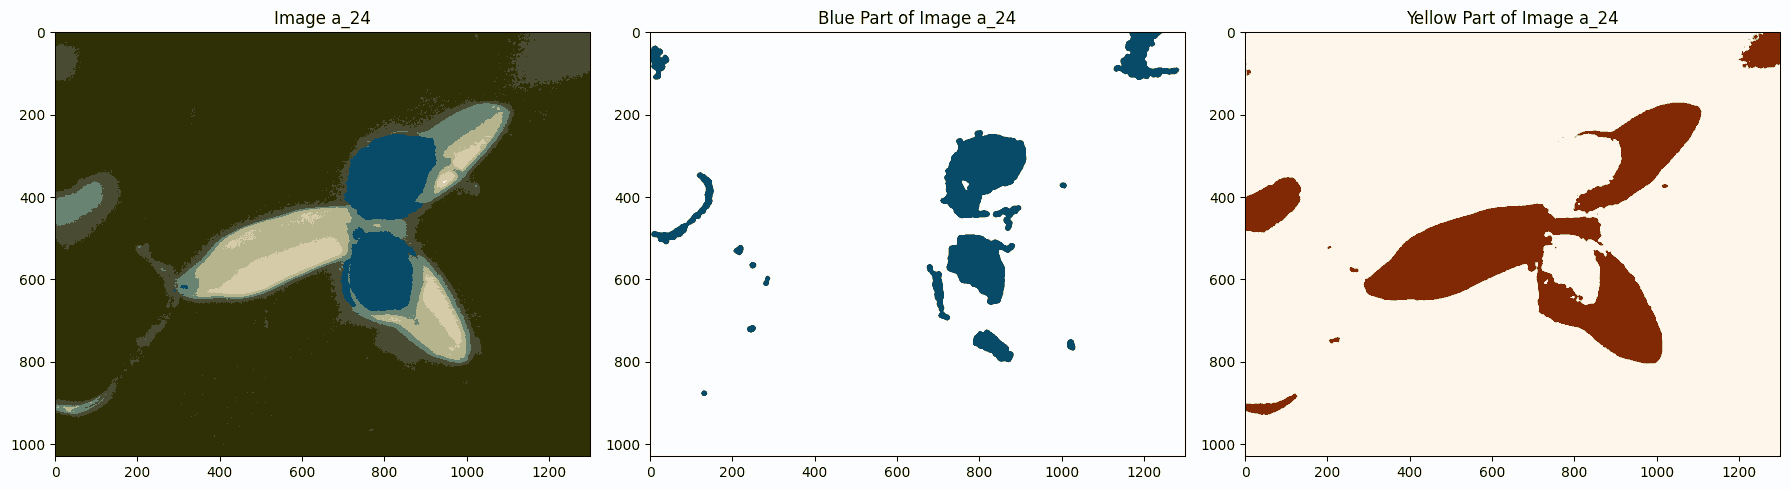
\includegraphics[width=0.95\textwidth]{Report/Images/Appendix Images/ColorSegments/Image24.png}
\caption{The series of segmented images (blue and yellow part) for the images 21-24} 
\label{fig:segment21-24}
\end{figure}
\begin{figure}[h!]
\centering
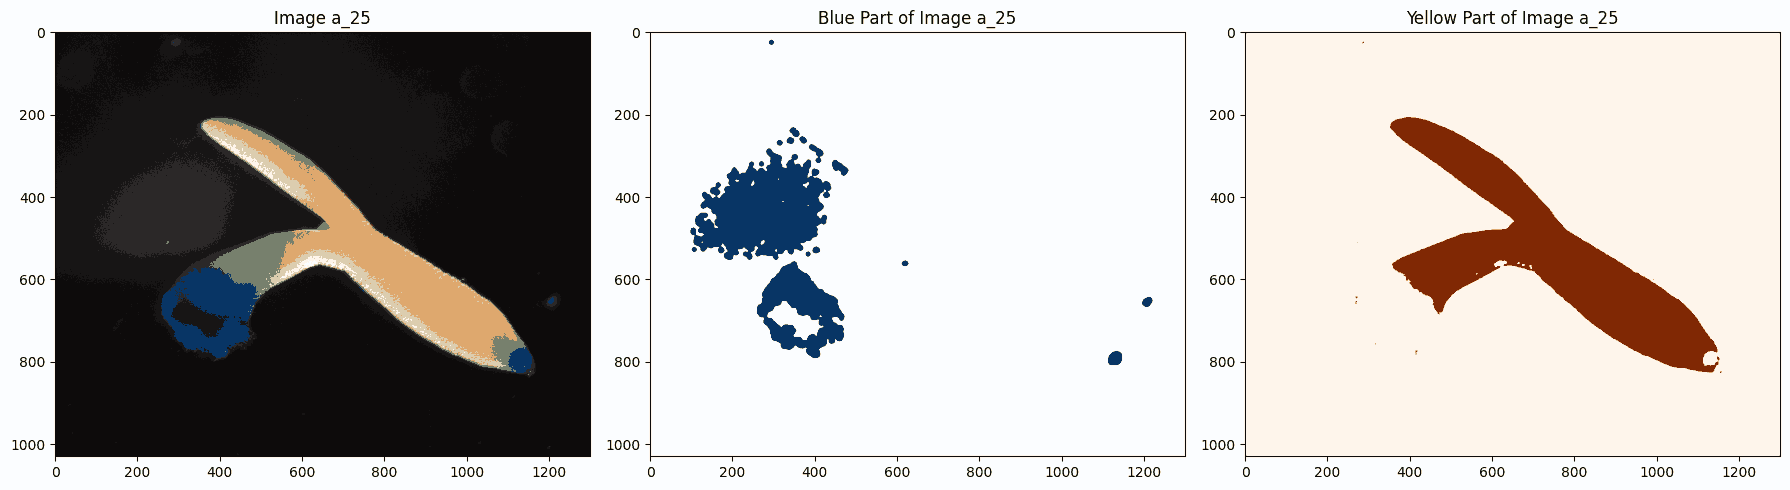
\includegraphics[width=0.95\textwidth]{Report/Images/Appendix Images/ColorSegments/Image25.png}
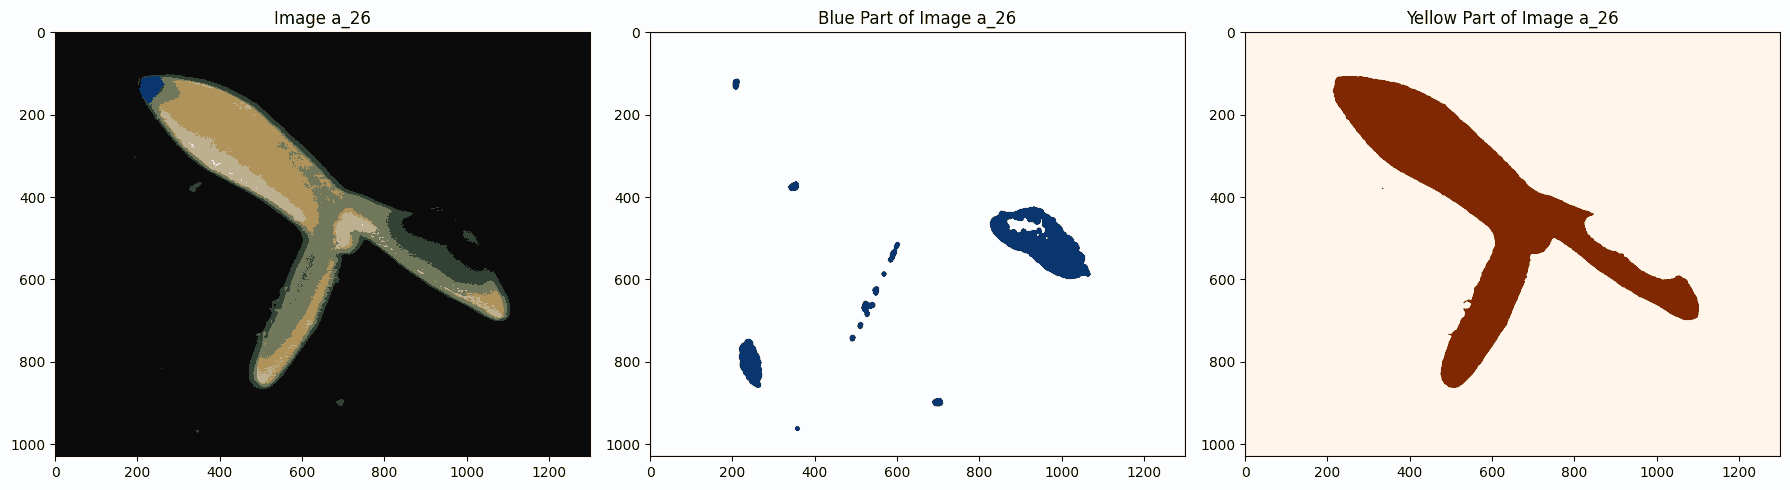
\includegraphics[width=0.95\textwidth]{Report/Images/Appendix Images/ColorSegments/Image26.png}
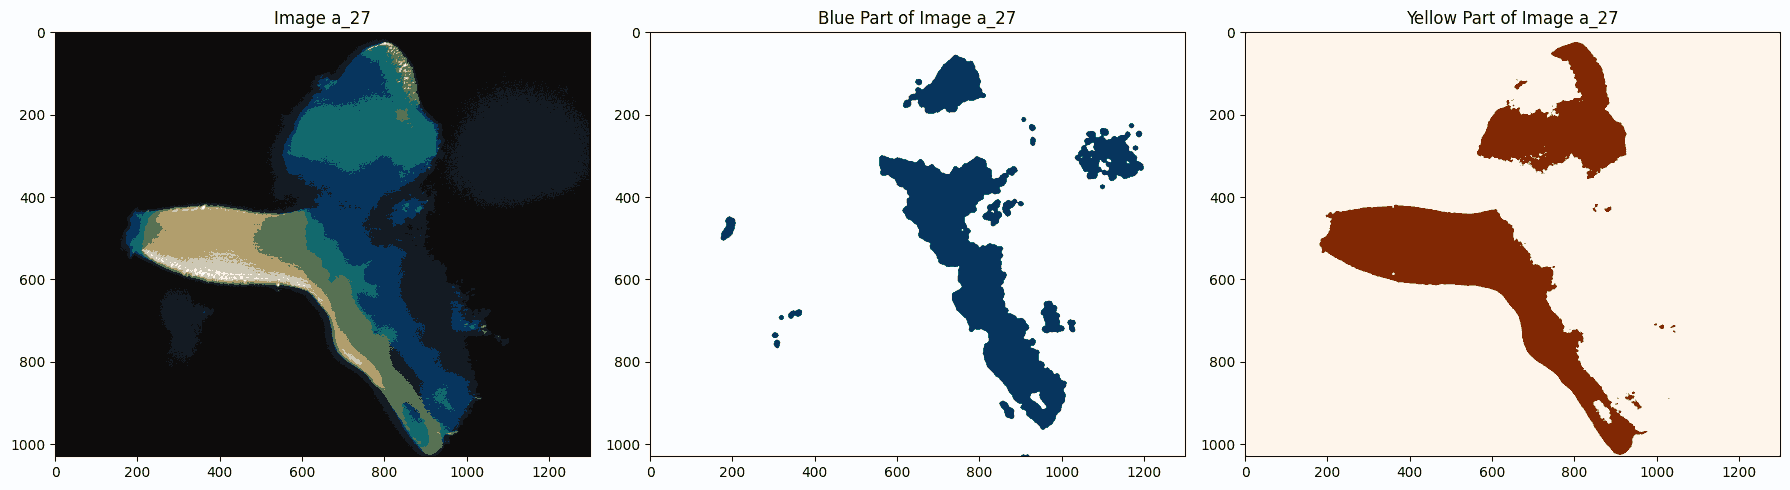
\includegraphics[width=0.95\textwidth]{Report/Images/Appendix Images/ColorSegments/Image27.png}
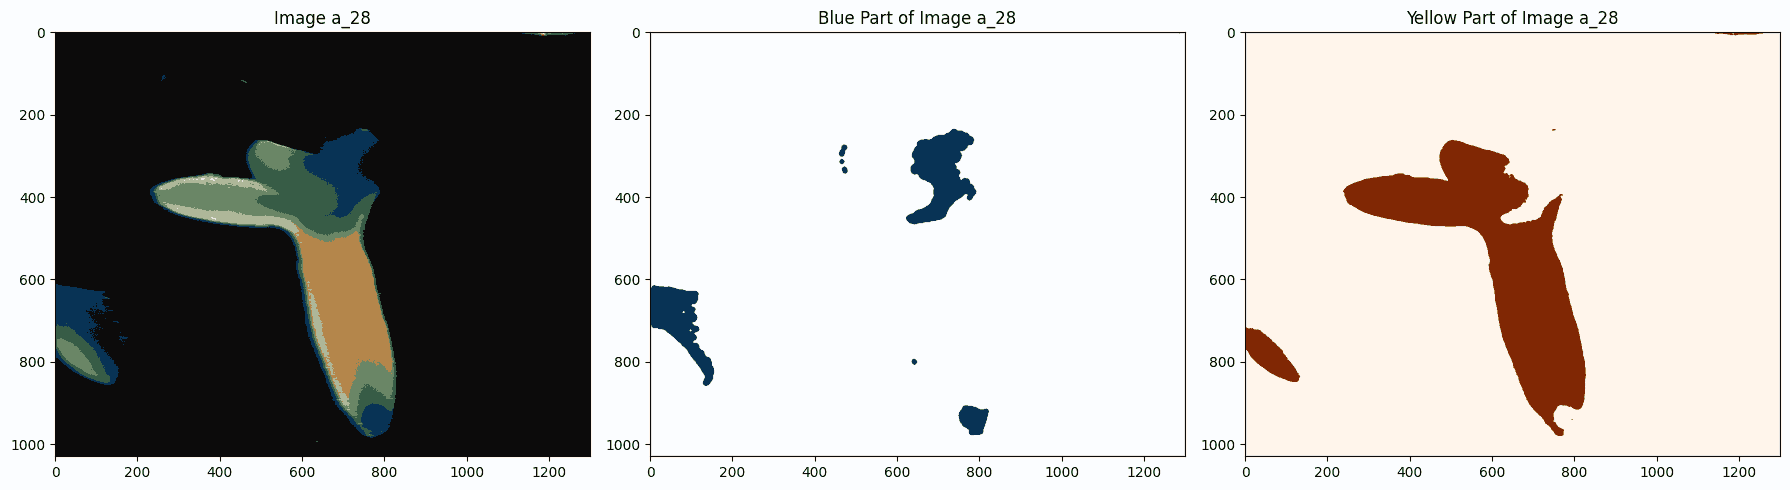
\includegraphics[width=0.95\textwidth]{Report/Images/Appendix Images/ColorSegments/Image28.png}
\caption{The series of segmented images (blue and yellow part) for the images 25-28} 
\label{fig:segment25-28}
\end{figure}
\begin{figure}[h!]
\centering
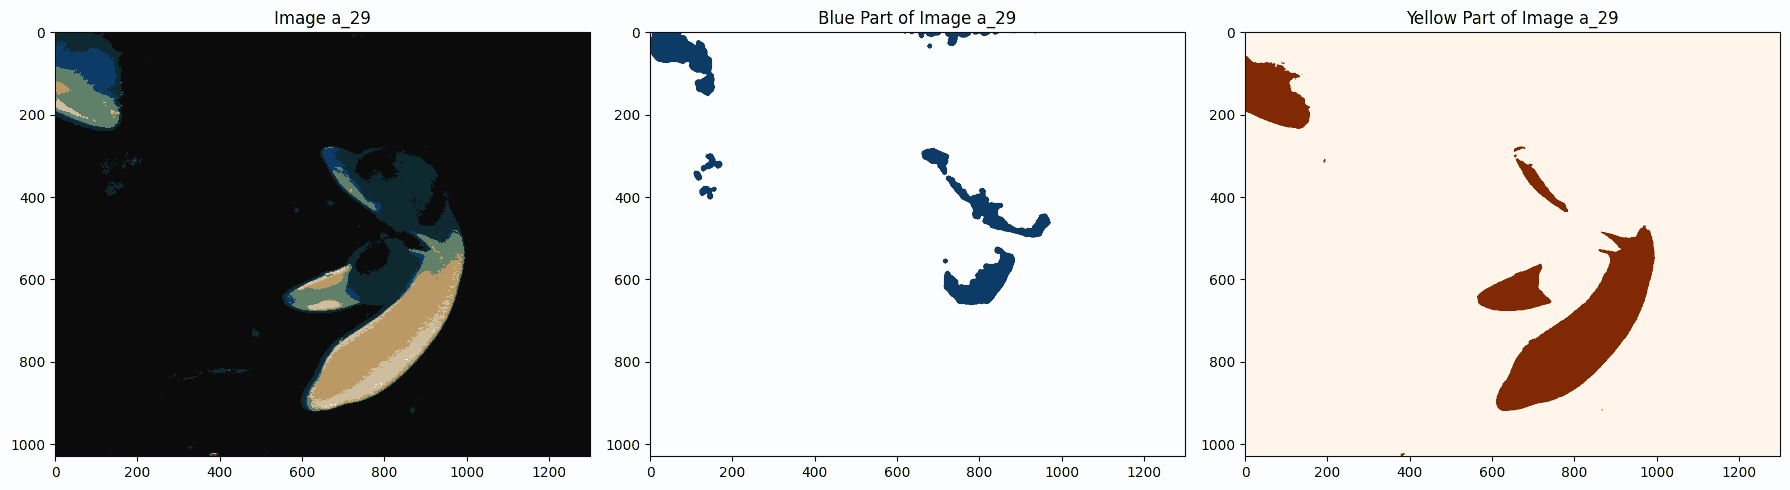
\includegraphics[width=0.95\textwidth]{Report/Images/Appendix Images/ColorSegments/Image29.png}
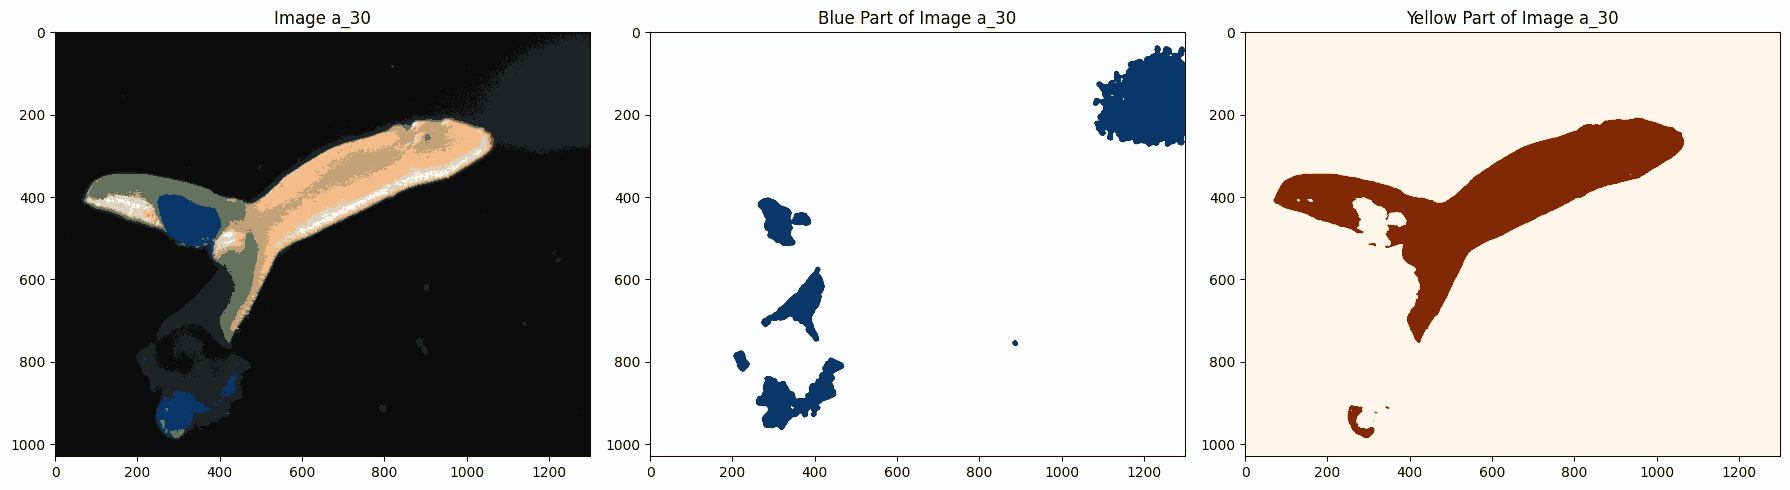
\includegraphics[width=0.95\textwidth]{Report/Images/Appendix Images/ColorSegments/Image30.png}
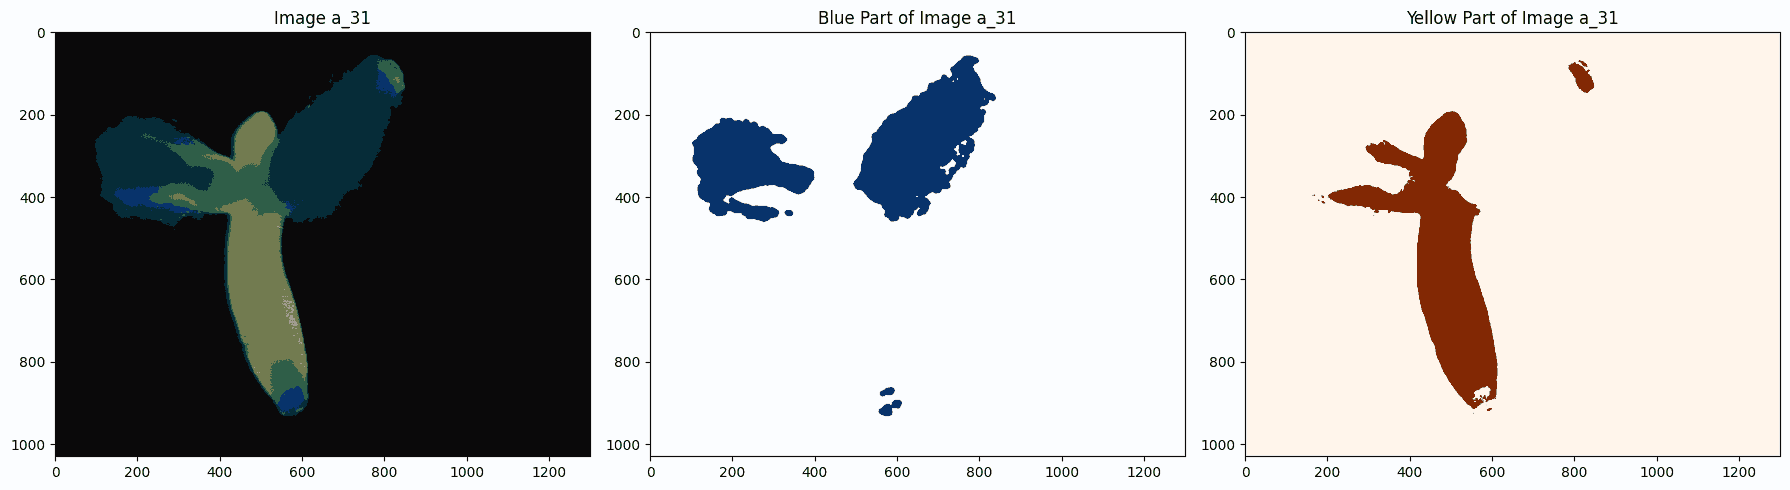
\includegraphics[width=0.95\textwidth]{Report/Images/Appendix Images/ColorSegments/Image31.png}
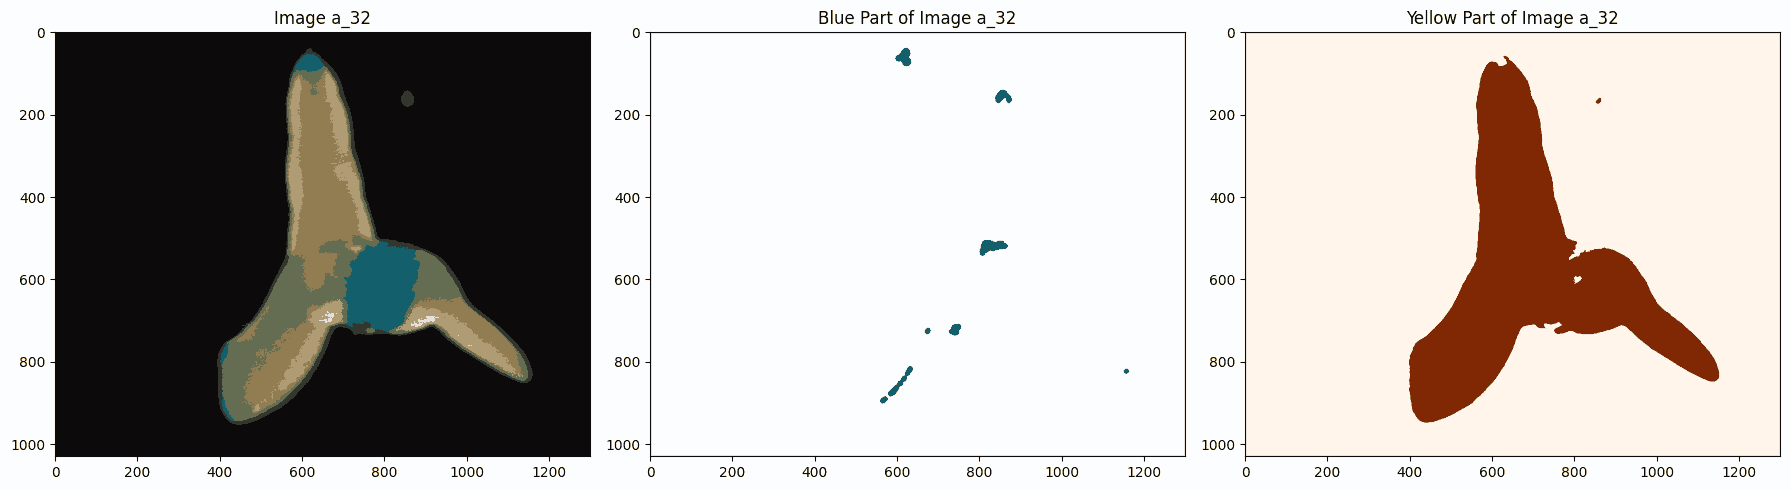
\includegraphics[width=0.95\textwidth]{Report/Images/Appendix Images/ColorSegments/Image32.png}
\caption{The series of segmented images (blue and yellow part) for the images 29-32} 
\label{fig:segment29-32}
\end{figure}
\begin{figure}[h!]
\centering
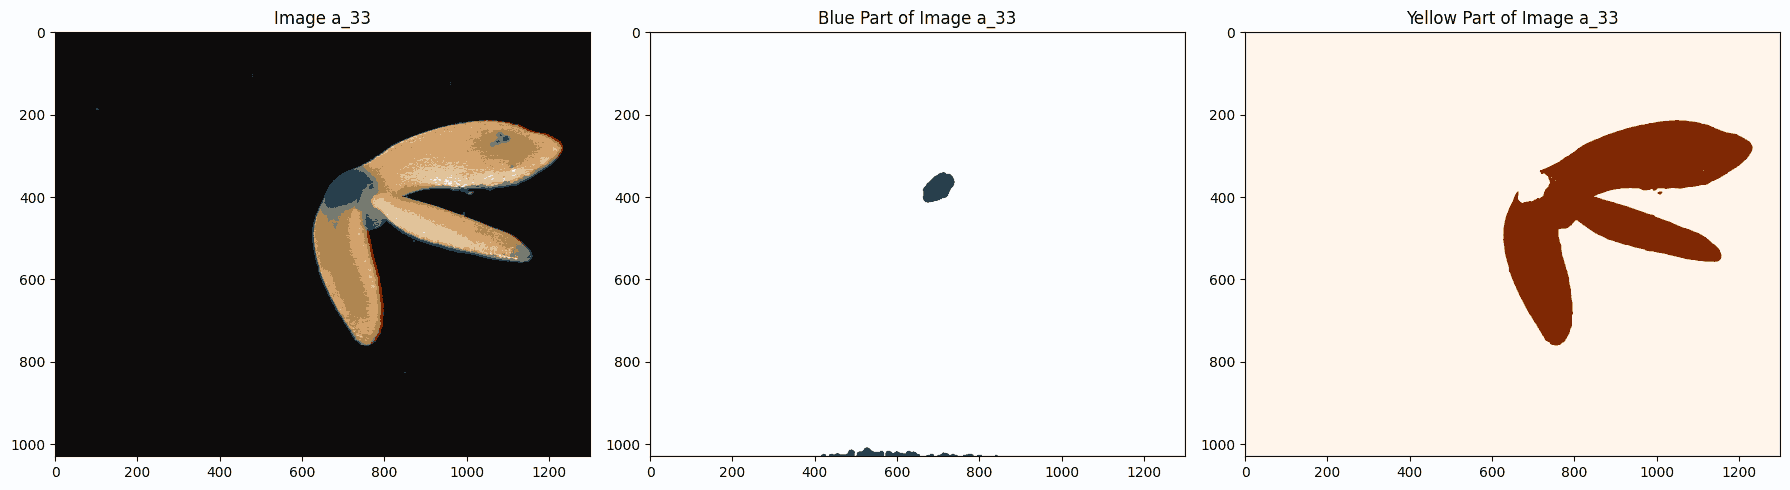
\includegraphics[width=0.95\textwidth]{Report/Images/Appendix Images/ColorSegments/Image33.png}
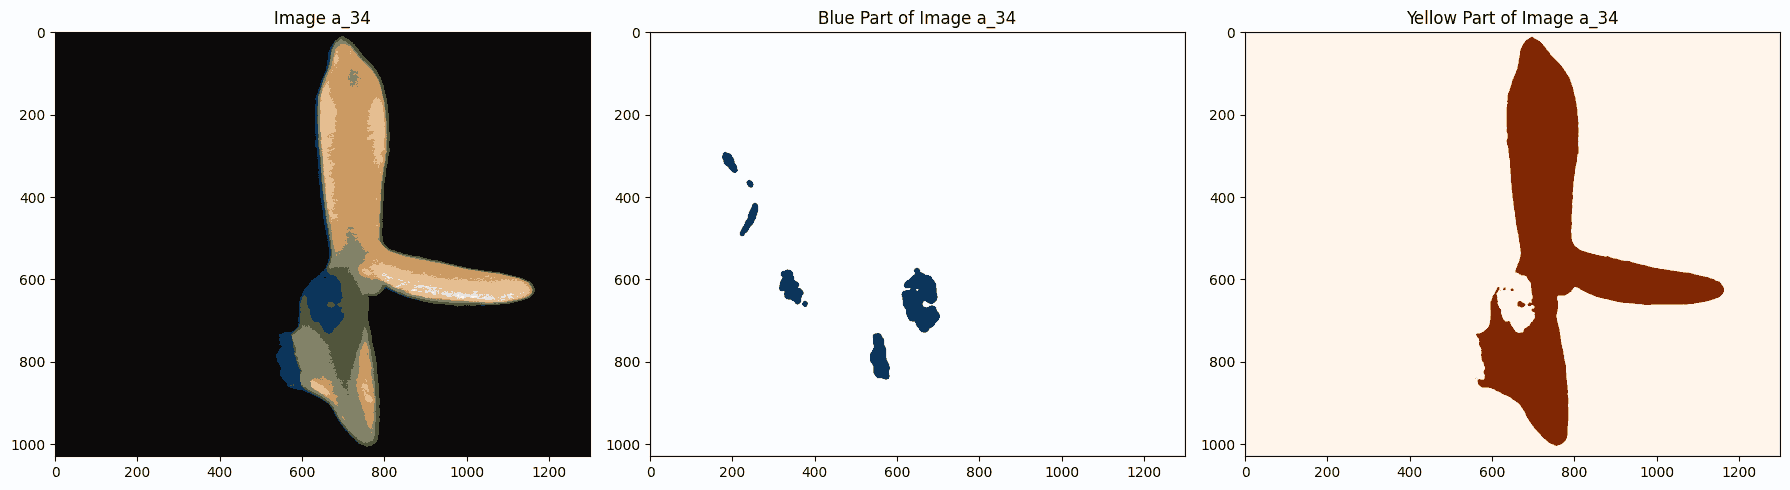
\includegraphics[width=0.95\textwidth]{Report/Images/Appendix Images/ColorSegments/Image34.png}
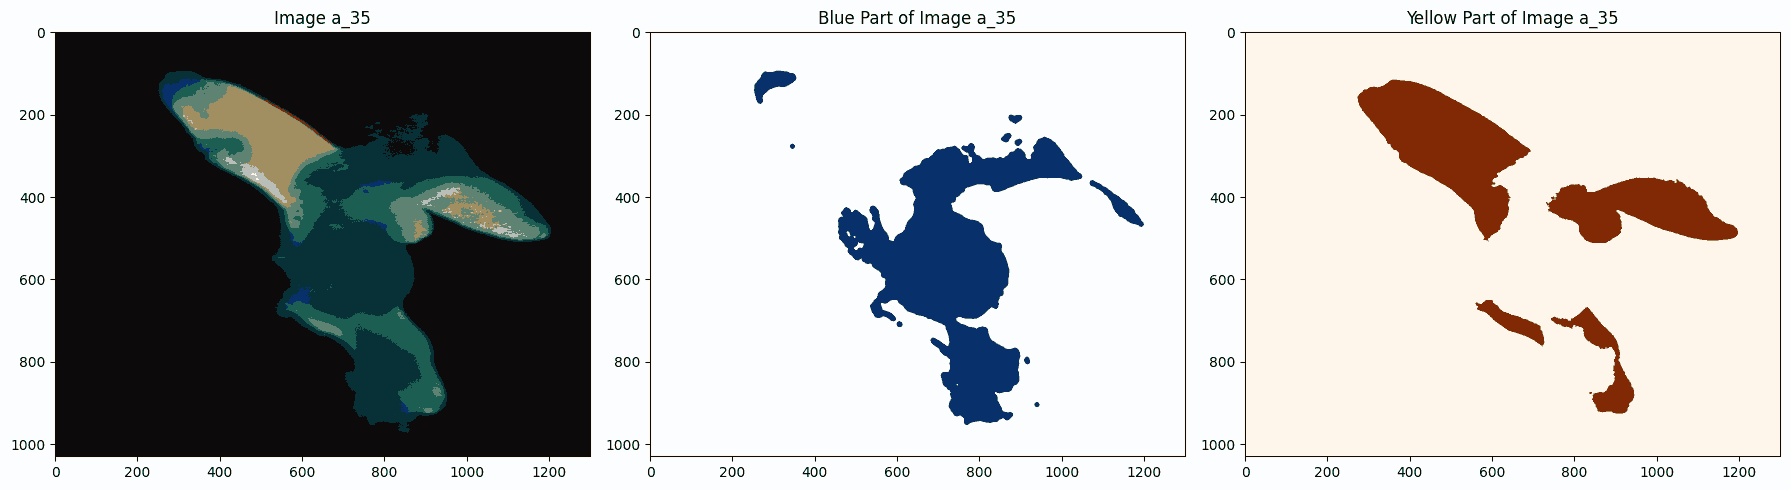
\includegraphics[width=0.95\textwidth]{Report/Images/Appendix Images/ColorSegments/Image35.png}
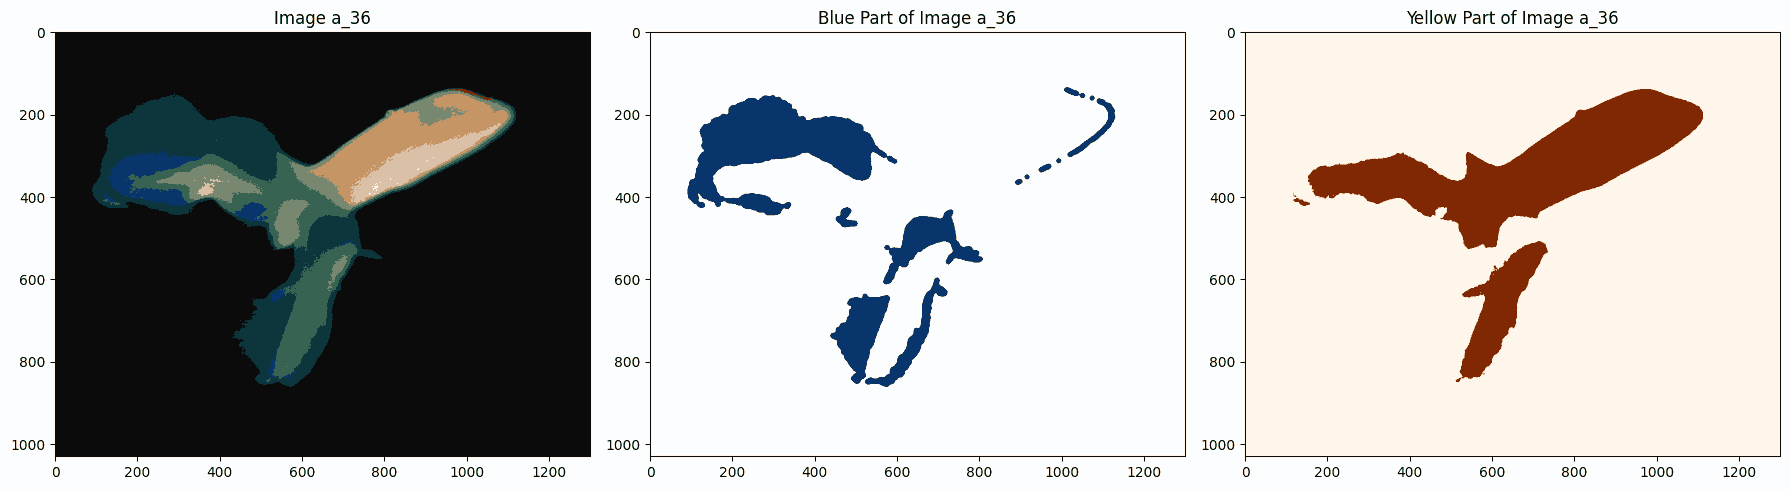
\includegraphics[width=0.95\textwidth]{Report/Images/Appendix Images/ColorSegments/Image36.png}
\caption{The series of segmented images (blue and yellow part) for the images 33-36} 
\label{fig:segment33-36}
\end{figure}
\begin{figure}[h!]
\centering
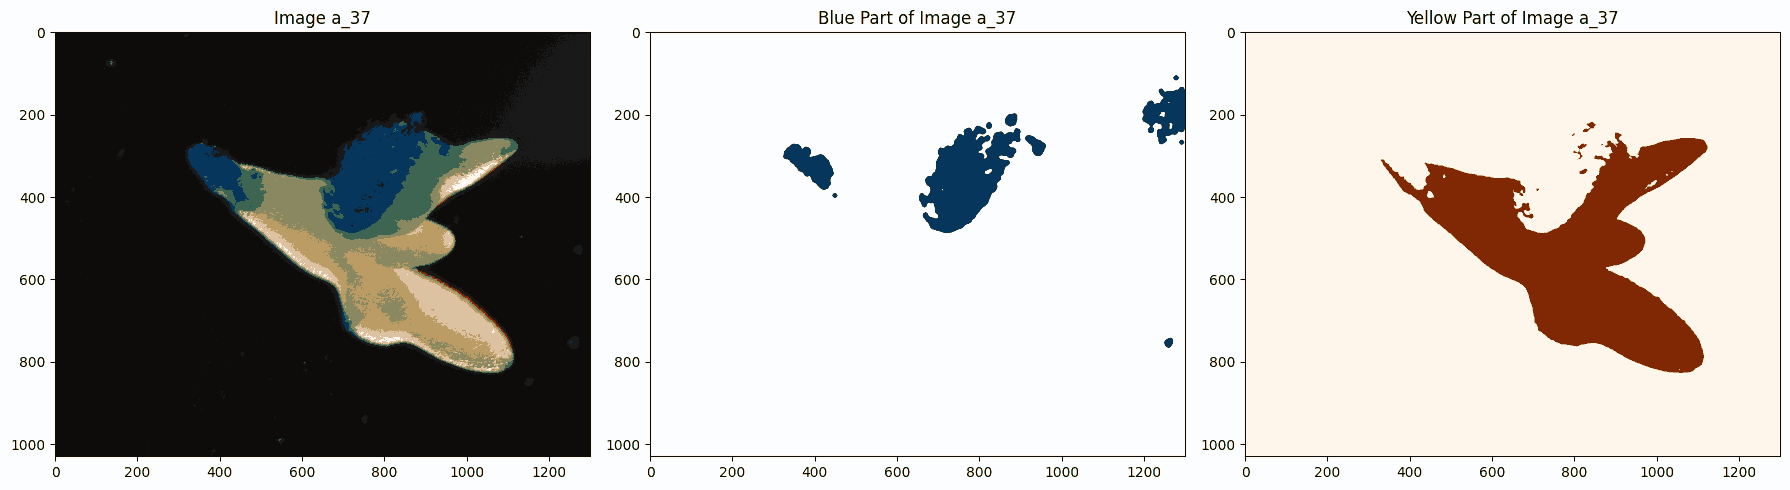
\includegraphics[width=0.95\textwidth]{Report/Images/Appendix Images/ColorSegments/Image37.png}
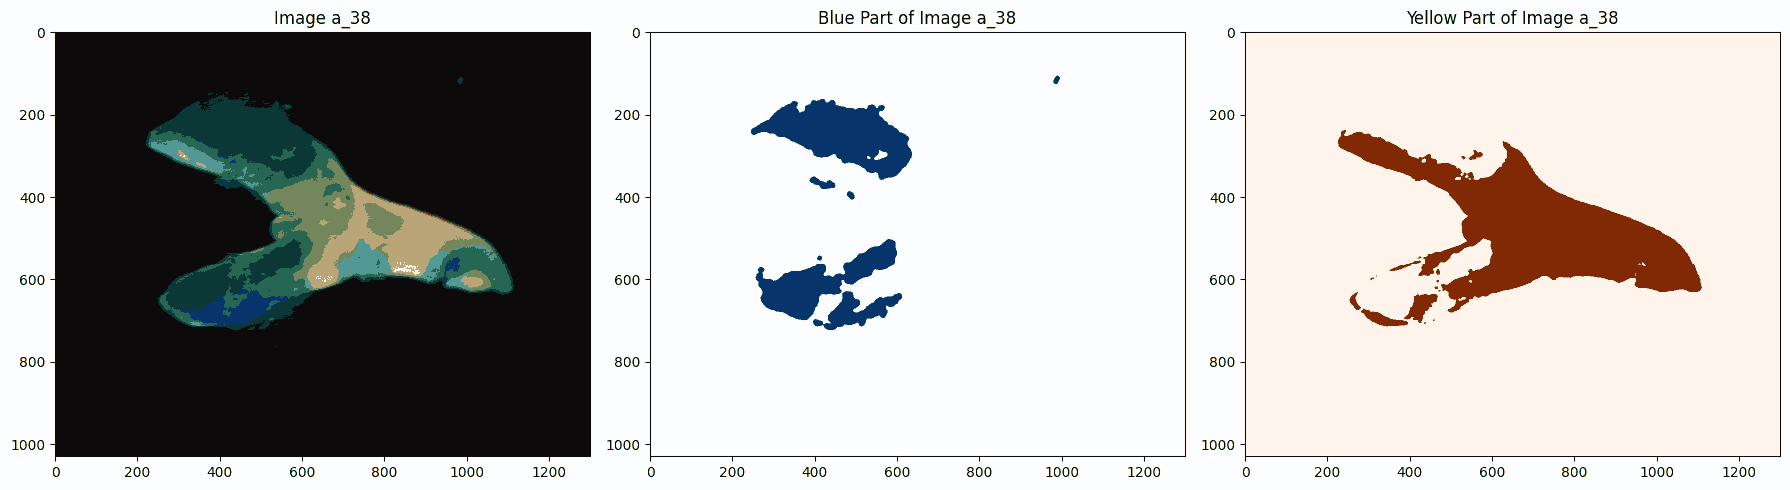
\includegraphics[width=0.95\textwidth]{Report/Images/Appendix Images/ColorSegments/Image38.png}
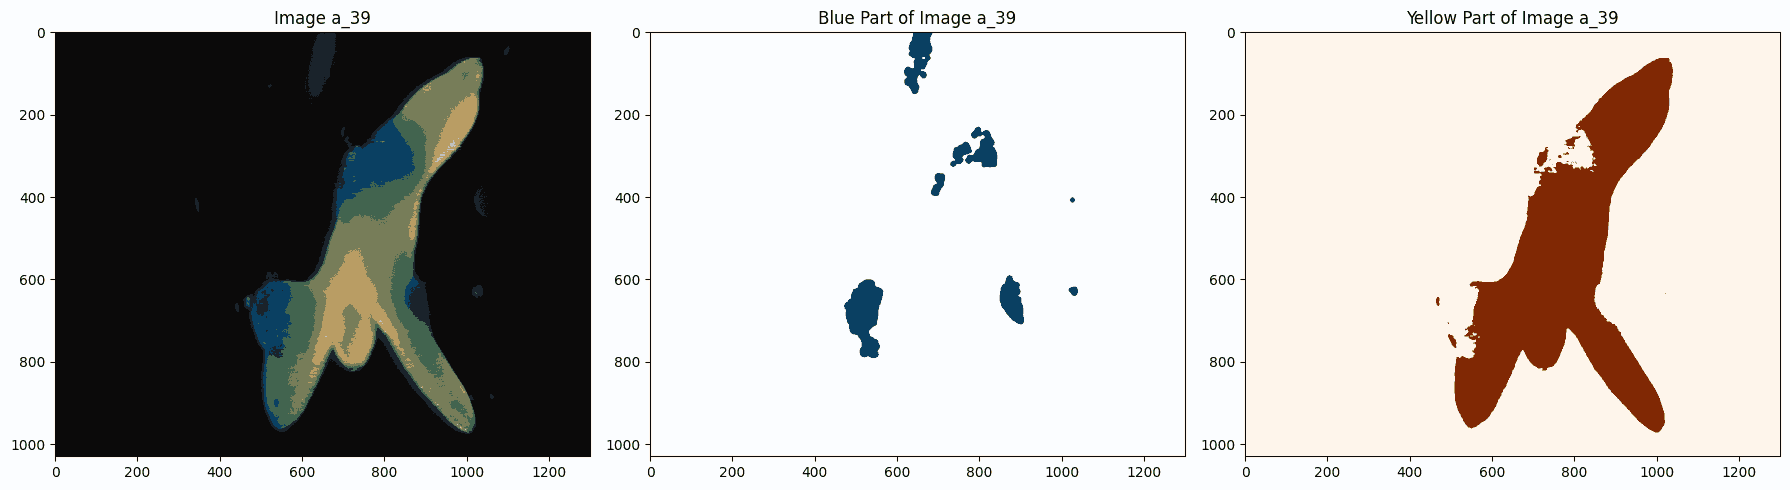
\includegraphics[width=0.95\textwidth]{Report/Images/Appendix Images/ColorSegments/Image39.png}
\includegraphics[width=0.95\textwidth]{Report/Images/Appendix Images/ColorSegments/Image40.png}
\caption{The series of segmented images (blue and yellow part) for the images 37-40} 
\label{fig:segment37-40}
\end{figure}
\begin{figure}[h!]
\centering
\includegraphics[width=0.95\textwidth]{Report/Images/Appendix Images/ColorSegments/Image41.png}
\includegraphics[width=0.95\textwidth]{Report/Images/Appendix Images/ColorSegments/Image42.png}
\includegraphics[width=0.95\textwidth]{Report/Images/Appendix Images/ColorSegments/Image43.png}
\includegraphics[width=0.95\textwidth]{Report/Images/Appendix Images/ColorSegments/Image44.png}
\caption{The series of segmented images (blue and yellow part) for the images 41-44} 
\label{fig:segment41-44}
\end{figure}
\begin{figure}[h!]
\centering
\includegraphics[width=0.95\textwidth]{Report/Images/Appendix Images/ColorSegments/Image45.png}
\includegraphics[width=0.95\textwidth]{Report/Images/Appendix Images/ColorSegments/Image46.png}
\includegraphics[width=0.95\textwidth]{Report/Images/Appendix Images/ColorSegments/Image47.png}
\includegraphics[width=0.95\textwidth]{Report/Images/Appendix Images/ColorSegments/Image48.png}
\caption{The series of segmented images (blue and yellow part) for the images 45-48} 
\label{fig:segment45-48}
\end{figure}
\begin{figure}[h!]
\centering
\includegraphics[width=0.95\textwidth]{Report/Images/Appendix Images/ColorSegments/Image49.png}
\includegraphics[width=0.95\textwidth]{Report/Images/Appendix Images/ColorSegments/Image50.png}
\includegraphics[width=0.95\textwidth]{Report/Images/Appendix Images/ColorSegments/Image51.png}
\includegraphics[width=0.95\textwidth]{Report/Images/Appendix Images/ColorSegments/Image52.png}
\caption{The series of segmented images (blue and yellow part) for the images 49-52} 
\label{fig:segment49-52}
\end{figure}
\begin{figure}[h!]
\centering
\includegraphics[width=0.95\textwidth]{Report/Images/Appendix Images/ColorSegments/Image53.png}
\includegraphics[width=0.95\textwidth]{Report/Images/Appendix Images/ColorSegments/Image54.png}
\includegraphics[width=0.95\textwidth]{Report/Images/Appendix Images/ColorSegments/image55.png}
\includegraphics[width=0.95\textwidth]{Report/Images/Appendix Images/ColorSegments/image56.png}
\caption{The series of segmented images (blue and yellow part) for the images 53-56} 
\label{fig:segment53-56}
\end{figure}
\begin{figure}[h!]
\centering
\includegraphics[width=0.95\textwidth]{Report/Images/Appendix Images/ColorSegments/image57.png}
\includegraphics[width=0.95\textwidth]{Report/Images/Appendix Images/ColorSegments/image58.png}
\caption{The series of segmented images (blue and yellow part) for the images 57-58} 
\label{fig:segment57-58}
\end{figure}
\end{document}